\documentclass[USenglish]{article}
% for 2-column layout use \documentclass[USenglish,twocolumn]{article}

\usepackage[utf8]{inputenc}				%(only for the pdftex engine)
%\RequirePackage[no-math]{fontspec}[2017/03/31]%(only for the luatex or the xetex engine)
\usepackage{xparse}  % Add this for older LaTeX compatibility
\usepackage[big,online]{dgruyter}	%values: small,big | online,print,work
\usepackage{lmodern}
\usepackage{microtype}
\usepackage[authoryear,round,sort&compress]{natbib}
\usepackage{graphicx}
\usepackage{amsmath}
\usepackage{booktabs}
\usepackage{caption}
\usepackage{subcaption}
\usepackage{float}
\usepackage[table]{xcolor}

% New theorem-like environments
\theoremstyle{dgthm}
\newtheorem{theorem}{Theorem}
\newtheorem{corollary}{Corollary}
\newtheorem{proposition}{Proposition}
\newtheorem{lemma}{Lemma}

\theoremstyle{dgdef}
\newtheorem{definition}{Definition}
\newtheorem{example}{Example}
\newtheorem{remark}{Remark}

\begin{document}

%%%--------------------------------------------%%%
	\articletype{Research Article}
	\received{November 6, 2024}
	\revised{Month DD, YYYY}
  \accepted{Month DD, YYYY}
  \journalname{Journal of Quantitative Analysis in Sports}
  \journalyear{2024}
  \journalvolume{XX}
  \journalissue{X}
  \startpage{1}
  \aop
  \DOI{10.1515/jqas-YYYY-XXXX}
%%%--------------------------------------------%%%

\title{Coaching DNA: Measuring Strategic Identity and Knowledge Transmission in the NFL}
\runningtitle{Coaching DNA in the NFL}

% Author information removed for blind peer review
%\author*[1]{Jon Williamson}
%\runningauthor{Williamson}
%\affil[1]{\protect\raggedright
%Knowledge Transmission in the NFL, e-mail: jon@williamsonconsultinggroup.com}

\abstract{We develop a framework to measure coaching ``DNA'' in the NFL: a coach's measurable strategic tendencies. Using XGBoost models on more than 600,000 plays from 2006--2024, we quantify four dimensions, offensive aggression, shotgun formation preference, tempo, and defensive aggression, each a residual from situation-adjusted predictions. The genes are stable coach traits, not team artifacts: coach identity explains several times the team's variance net of a permutation null, and they travel across team changes (composite offensive aggression $r=0.57$). Because a leaguewide baseline drifts over our window, we keep the genes absolute but control for the contemporary-group (within-season) baseline in inference. Under this control, offensive aggression ($r=0.18$) and defensive aggression ($r=0.15$) predict context-adjusted Coach WAR, while shotgun and tempo do not, and within coaches higher aggression still adds wins, an edge that has narrowed as it diffused. Neither mentor performance ($r=0.12$) nor offensive aggression transmits to prot\'{e}g\'{e}s. Schematic identity does, through the offensive-coordinator apprenticeship (a mentor's own coordinators $r=0.41$; direct coordinator-to-head-coach $r=0.63$), as does defensive aggression ($r=0.56$). The trait that wins is personal; the trait that transmits does not by itself win: coaching trees propagate systems, not success or risk tolerance.}

\keywords{NFL coaching, coaching DNA, coaching trees, strategic identity, competitive advantage}

\maketitle

\section{Introduction}

Fourth-down analytics consistently show that aggressive coaches win more games \citep{romer2006,yam2019}. Teams that ``go for it'' on fourth down in marginal situations would gain approximately 0.4 additional wins per season on average \citep{yam2019}. Expected points models demonstrate that punting from midfield often surrenders value \citep{burke2009}. These findings raise a deeper question in competitive strategy: if aggressive decisions are individually optimal, does their advantage persist once every team adopts them? 

NFL coaching is among the highest-stakes decision-making environments in professional sports. Head coaches command salaries that average several million dollars and reach \$20 million for the highest-paid \citep{sportico2024}, and their individual in-game choices are dissected in granular detail by analysts and fans. Yet how a coach is characterized, as aggressive, conservative, run-heavy, or innovative, still rests largely on narrative and reputation rather than measurement. We lack an objective, decision-level characterization of even a portion of a coach's strategic tendencies.

These tendencies surface in dozens of observable choices every game: whether to go for it on fourth down, whether to run from shotgun or under center, how fast to snap the ball, how many defenders to send after the quarterback. Each choice reflects a coach's strategic identity, their ``DNA.'' But the tendencies are hard to measure objectively, hard to separate from forced circumstance, and hard to classify as stable traits versus situational adaptations. Providing that characterization is the goal of this project.

\subsection{Measuring Coaching Philosophy}

We propose a general framework for quantifying coaching tendencies across multiple strategic dimensions. For each decision type, we train a machine learning model on situational features (game state, field position, score, time, environment) to predict what the ``average'' coach would do in identical circumstances. Depending on the decision, this model is a classifier (for discrete choices such as going for it on fourth down) or a regressor (for continuous behaviors such as seconds between snaps). In either case, a coaching gene is the systematic deviation between a coach's actual decisions and these situation-adjusted predictions:

\begin{equation}
\text{Gene}_c = \text{Actual Rate}_c - \text{Predicted Rate}_c
\end{equation}

This residual approach isolates genuine strategic tendency from forced circumstance. A coach who goes for it on fourth down frequently only because they are always trailing is not truly aggressive. Only the \emph{excess} tendency beyond what the situation demands is attributed to coaching philosophy. We apply this framework to four dimensions of coaching DNA:

\begin{itemize}
\item \textbf{Offensive Aggression}: a composite of four sub-components, namely fourth-down decisions, pass-run balance, deep passing tendency, and two-point conversion attempts. This is the dimension with the strongest theoretical prior for predicting performance, since analytics research finds aggressive fourth-down decisions are frequently expected-value optimal \citep{romer2006,burke2009}.
\item \textbf{Shotgun formation preference}: a single gene capturing whether coaches run more or less shotgun than game context predicts, reflecting offensive system design independent of situational necessity.
\item \textbf{Tempo}: a composite of no-huddle usage and pace (seconds between plays, with faster-than-expected scored positively), measuring how fast an offense operates.
\item \textbf{Defensive aggression}: a composite of box stacking, pass rush intensity, and man-versus-zone coverage tendency, measured at the team level from 2016 onward (man/zone from 2018).
\end{itemize}
Three of the four dimensions are composites of their sub-components and shotgun preference is a single gene; together they profile coaching DNA across both sides of the ball. These four are the genes we examine here, not an exhaustive catalog of coaching behavior: other genes surely exist, and the framework extends to any decision with enough plays to model. A first question is whether such measures are stable traits that belong to coaches rather than artifacts of the teams they happen to coach.

\subsection{The Coaching Tree Framework}

When NFL teams hire head coaches, pedigree frequently influences decisions. Coordinators from successful organizations receive premium consideration, with the implicit assumption that working under successful coaches transfers strategic expertise and winning approaches. The coaching tree hypothesis makes three testable predictions: (1) successful mentors produce successful prot\'{e}g\'{e}s, (2) strategic tendencies transmit through apprenticeship, and (3) coaching DNA persists through promotion from coordinator to head coach. We directly test all three.

\subsection{WAR as the Measure of Coaching Success}

To test whether coaching genes relate to success, we need a measure of coaching quality that separates a coach's contribution from inherited circumstances, since win-loss records confound coaching ability with roster talent, strength of schedule, and luck. We adopt Coach Wins Above Replacement (Coach WAR), a context-adjusted estimate of the wins a coach adds relative to a replacement-level alternative, developed and validated on held-out coaches in companion work \citep{williamson2026war}. Using Coach WAR as the outcome lets us ask whether a coach's strategic DNA predicts winning once roster quality and circumstance are accounted for.

\section{Literature Review}

The study of coaching decision-making in the NFL has focused primarily on conservative bias. \citet{romer2006} demonstrated that NFL coaches punt too frequently on fourth down, forgoing positive-expected-value conversion attempts, a robust and widely cited finding. \citet{yam2019} extended this work with causal estimates, finding that teams adopting more aggressive fourth-down strategies would gain approximately 0.4 wins per season. \citet{horowitz2014} confirmed the persistence of the fourth-down puzzle using different statistical methods, while \citet{burke2009} generalized the finding through expected points models showing that conservative play-calling surrenders value across a range of game situations. Collectively, this literature establishes that aggressive coaching decisions are often optimal in isolation, but does not address whether the advantage persists as adoption spreads.

A parallel literature has sought to quantify team quality more broadly. \citet{schatz2003} developed DVOA (Defense-adjusted Value Over Average), one of the first publicly available metrics for evaluating team performance adjusted for opponent quality. These metrics, however, are fundamentally team-level \emph{outcome} measures that combine the on-field performance of players, coordinators, and coaching staffs. They capture how well a team performed, not the strategic choices behind that performance, and so cannot separate a head coach's philosophy from the talent executing it. On coaching careers specifically, \citet{goff2006} identified a managerial life cycle in the NFL, in which coaches tend to perform best in their early years and decline over time, suggesting that coaching effectiveness is not static and may interact with organizational context. What remains missing is a framework that measures coaching \emph{decision tendencies} rather than outcomes, namely what coaches choose to do beyond what the situation demands, decomposed into dimensions that can be tracked across time, relationships, and career transitions.

The competitive dynamics of strategic adoption have been studied extensively outside sports. \citet{rogers2007} formalized the S-curve pattern of innovation diffusion, in which early adopters gain outsized advantages that erode as the innovation becomes mainstream. Because the analytics literature establishes that aggressive tactics are expected-value positive, this framework predicts that aggressive tactics should follow a similar trajectory: they provide a competitive edge while rare, an edge that erodes as analytics-driven decision-making becomes universal. However, this prediction has not been empirically tested in the coaching context.

Several gaps emerge from this literature. Most fundamentally, no prior work offers a general framework that decomposes coaching behavior into multiple measurable genes spanning both sides of the ball; existing studies treat aggression, and chiefly fourth-down aggression, in isolation rather than as one dimension of a broader strategic identity. Within that narrower lens, specific questions also remain open. No studies have examined how the offensive aggression-performance relationship evolves temporally as analytics disseminate and defenses adapt. Offensive aggression persistence within coaches, distinguishing stable traits from situational tactics, has not been systematically analyzed. Coaching tree effects have not been tested using context-adjusted performance metrics that control for inherited roster quality. Whether strategic philosophies genuinely transmit from mentors to prot\'{e}g\'{e}s, and which dimensions show transmission, remains unexamined.

\section{Methods}

\subsection{Data}

Our analysis integrates three complementary datasets spanning nearly two decades of NFL football. The primary dataset consists of play-by-play records for every offensive snap from the 2006 through 2024 seasons, obtained through the \texttt{nfl\_data\_py} package. This yields more than 600,000 analyzable plays with complete situational information (down, distance, field position, score differential, time remaining, and environmental conditions). The exact number of plays entering each model varies with the decision being modeled. The 2006 starting point is determined by data availability, particularly for air yards data required for our deep passing analysis.

The coaching data comes from career histories scraped from Pro Football Reference, giving complete position-by-position timelines for each coach. From these we build the coaching tree, the network of mentor-protégé relationships on which our inheritance analyses rest, matched on a year-aware canonical franchise key so that relocations are handled correctly. We scope the tree to the modern era (1970--2025): 325 coaches connected by 1{,}425 documented mentor-protégé relationships, where a coordinator or position coach is counted as a protégé of any head coach they worked under for at least one season. Coach backgrounds (offensive, defensive, or other) are assigned by pattern matching on the role titles a coach held before becoming a head coach. The gene measures described below, by contrast, require play-by-play data and so exist only for 2006--2024, a window in which 185 of these coaches were active; analyses that need a gene value are restricted accordingly.

Performance metrics come from a separate Wins Above Replacement (WAR) calculation that estimates each head coach's contribution to team success relative to a replacement-level alternative \citep{williamson2026war}. This dataset contains 1,637 coach-year observations spanning the modern era (1970--2024), which we merge with our gene measures on a canonicalized coach name and season, logging attrition. The merge yields 608 coach-year observations for offensive genes (offensive aggression, shotgun, tempo) and 282 for defensive aggression (2016--2024 only), covering 124 unique head coaches; the 33 unmatched gene coach-years (31 coaches) are all partial-season interim stints (none a full 16-game season). Coach WAR does not score these stints because they lack a replacement-level baseline, and in their gene values they do not differ systematically from the retained sample. We classify these coach-years by background as 310 offensive (51.2\%) and 251 defensive (41.4\%), with 45 (7.4\%) having substantial experience on both sides of the ball; the offensive-versus-defensive comparisons that follow use the 561 cleanly classified observations.

\subsection{Measuring Coaching Genes}
\label{sec:genes}

Each gene measures systematic deviation from expected decision-making. Rather than using raw frequencies, which confound individual tendencies with situational factors, we train machine learning models to predict baseline behavior and measure how much a coach or team deviates from these predictions. Across the four gene dimensions we fit ten component models, one per observable decision, and form the genes from their residuals. Offensive Aggression, tempo, and defensive aggression are \emph{composite} genes built from several component models, while shotgun preference is a single-model gene; Table~\ref{tab:gene_architecture} maps the ten models to the four genes.

We use gradient-boosted decision trees (XGBoost) for every component model because they are consistently the strongest performers on tabular, point-in-time prediction of this kind: with heterogeneous structured features rather than images or text, gradient-boosted trees outperform deep networks \citep{chen2016,grinsztajn2022}. Each model is a classifier or a regressor depending on its target, but the residual definition of a gene (Equation~1) is identical in both cases. Every model is trained on situational features alone and excludes season, week, and coach identity, so the baseline reflects what the average coach would do in identical circumstances and our analyses of temporal evolution and individual differences are not confounded. Hyperparameters are tuned per model by randomized search (100 iterations), with 5-fold stratified cross-validation for classifiers and KFold for regressors.

\begin{table}[H]
\caption{The four coaching genes and their ten component models}
\label{tab:gene_architecture}
\scriptsize
\begin{tabular}{lllccc}
\toprule
\textbf{Gene} & \textbf{Component model} & \textbf{Type} & \textbf{Attribution} & \textbf{Features} & \textbf{Seasons} \\
\midrule
\multirow{4}{*}{Offensive Aggression (composite)} & Fourth-down decision & Classifier & Head coach & 16 & 2006--2024 \\
 & Run vs.\ pass & Classifier & Head coach & 16 & 2006--2024 \\
 & Pass target (deep) & Classifier & Head coach & 17 & 2006--2024 \\
 & Two-point conversion & Classifier & Head coach & 16 & 2006--2024 \\
\midrule
Shotgun (single) & Shotgun formation & Classifier & Head coach & 16 & 2006--2024 \\
\midrule
\multirow{2}{*}{Tempo (composite)} & No-huddle & Classifier & Head coach & 18 & 2006--2024 \\
 & Pace (seconds/play) & Regressor & Head coach & 15 & 2006--2024 \\
\midrule
\multirow{3}{*}{Defensive aggression (composite)} & Box stacking & Regressor & Team-year & 15 & 2016--2024 \\
 & Pass rush & Regressor & Team-year & 17 & 2016--2024 \\
 & Man coverage & Classifier & Team-year & 20 & 2018--2024 \\
\bottomrule
\end{tabular}
\\[2pt]
{\scriptsize The Features column gives the number of stability-selected predictors each model retains from the shared candidate pool (Table~\ref{tab:model_features}). Offensive Aggression, tempo, and defensive aggression are composites of their component genes; shotgun is a single component.}
\end{table}

\begin{table}[H]
\caption{Shared candidate feature pool for the component models}
\label{tab:model_features}
\scriptsize
\begin{tabular}{lc}
\toprule
\textbf{Feature Category} & \textbf{Models} \\
\midrule
\textbf{Game State (13 features)} & All \\
\quad Score differential, quarter, seconds remaining, & \\
\quad timeouts remaining (both teams), down, distance & \\
\midrule
\textbf{Field Position (5 features)} & All except Two-Point \\
\quad Yard line, goal-to-go, side of field, distance, down & \\
\midrule
\textbf{Environmental (6 features)} & All \\
\quad Home/away, division game, roof, surface, temp, wind & \\
\midrule
\textbf{Drive Context (3 features)} & All \\
\quad Drive play count, drive first downs, net yards & \\
\midrule
\textbf{Vegas Lines (2 features)} & All \\
\quad Spread, total & \\
\midrule
\textbf{Pre-snap indicators (2 features)} & Defensive models \\
\quad Shotgun, no-huddle (observed pre-snap offense) & \\
\bottomrule
\end{tabular}
\\[2pt]
{\scriptsize Offensive models draw on up to 26 candidates (21 for two-point, which omits field position); defensive models add the two pre-snap indicators for 28. Each model's stability-selected subset is listed in Table~\ref{tab:gene_architecture}.}
\end{table}

From the candidate pool in Table~\ref{tab:model_features}, each model retains only a stability-selected subset of features (see Section~\ref{sec:pipeline}), reducing the 21--28 candidates to 15--20 stable predictors per model and guarding against overfitting collinear context variables.

Model performance varies across the ten components and is summarized for all of them in Table~\ref{tab:all_models}. Under grouped resampling that holds out whole team-years (so no team's plays appear in both training and evaluation), the classifiers range from man coverage (AUC $0.68$) up to fourth-down decisions (AUC $0.98$), while the regressors explain a more modest share of variance. In every case, situational factors explain most of the decision-making variance, leaving a smaller residual that we attribute to coaching philosophy.

\begin{table}[H]
\caption{Predictive Model Performance (Nadeau-Bengio corrected resampling)}
\label{tab:all_models}
\scriptsize
\textbf{Classifiers (AUC)}\\[2pt]
\begin{tabular}{llccc}
\toprule
\textbf{Gene} & \textbf{Model} & \textbf{AUC} & \textbf{95\% CI} & \textbf{Seasons} \\
\midrule
\multirow{4}{*}{Offensive Aggression} & 4th Down Decision & 0.975 & [0.973, 0.976] & 2006--2024 \\
 & Run vs Pass & 0.784 & [0.782, 0.786] & 2006--2024 \\
 & Pass Target & 0.734 & [0.731, 0.736] & 2006--2024 \\
 & Two-Point Conversion & 0.927 & [0.914, 0.940] & 2006--2024 \\
\midrule
Shotgun & Shotgun Formation & 0.807 & [0.802, 0.812] & 2006--2024 \\
Tempo & No-Huddle & 0.766 & [0.758, 0.775] & 2006--2024 \\
Def.\ Aggression & Man Coverage & 0.680 & [0.673, 0.687] & 2018--2024 \\
\bottomrule
\end{tabular}
\\[6pt]
\textbf{Regressors (RMSE and $R^2$)}\\[2pt]
\begin{tabular}{llcccc}
\toprule
\textbf{Gene} & \textbf{Model} & \textbf{RMSE} & \textbf{95\% CI} & \textbf{$R^2$ [95\% CI]} & \textbf{Seasons} \\
\midrule
Tempo & Pace (seconds) & 11.08 & [11.04, 11.11] & 0.428 [0.424, 0.432] & 2006--2024 \\
\multirow{2}{*}{Def.\ Aggression} & Box Stacking & 0.811 & [0.801, 0.820] & 0.422 [0.411, 0.433] & 2016--2024 \\
 & Pass Rush & 0.811 & [0.793, 0.829] & 0.055 [0.051, 0.059] & 2016--2024 \\
\bottomrule
\end{tabular}
\\[2pt]
{\scriptsize Point estimates and 95\% CIs are Nadeau-Bengio corrected resampled-$t$ intervals \citep{nadeau2003} over $J=50$ grouped resamples (GroupShuffleSplit holding out whole team-years, so no team appears in both train and test). The corrected variance inflates the naive resample variance to account for the overlap among resampled training sets. RMSE units differ by target: seconds for pace, players for box stacking and pass rush. The low pass-rush $R^2$ reflects that pass-rusher counts are only weakly predictable from pre-snap context, leaving more of their variation to coaching tendency.}
\end{table}

\subsubsection{Offensive Aggression Gene}

Offensive Aggression is a composite of four component models, each predicting a discrete in-game decision: going for it on fourth down, passing versus running, targeting beyond the first-down marker versus at or short of it (air yards exceeding the yards to go), and attempting a two-point conversion versus an extra point. For each coach-year, we calculate component-specific offensive aggression scores using Equation~1, where $c$ indexes the four components. The composite is a \emph{reliability-weighted} average of the four standardized component scores: each component is weighted by its reliability, the share of its variance that is true between-coach signal rather than sampling noise, so that one measured from few plays contributes less. We estimate these reliabilities with a DerSimonian-Laird random-effects model \citep{dersimonian1986}, detailed in Section~\ref{sec:pipeline}. We treat offensive aggression as a \emph{formative} construct. The four components are distinct facets that jointly constitute aggressive decision-making rather than indicators of a single latent trait (they are only weakly inter-correlated), so we report component-level results alongside the composite throughout.

\subsubsection{Shotgun Formation Gene}

We train an XGBoost classifier to predict whether each play will be run from shotgun formation, using the offensive candidate feature set (Table~\ref{tab:model_features}, stability-selected to 16 features). The shotgun gene for each coach-year is the difference between actual and predicted shotgun rates, reliability-shrunk toward the league mean (so low-play coach-years are not over-trusted) and z-scored across all coach-years for comparability; because head-coach seasons carry ample plays, this shrinkage is small in practice. This gene captures formation preference independent of game context and is attributed to head coaches, yielding 638 coach-year observations across 2006--2024.

\subsubsection{Tempo Gene}

The tempo gene combines two sub-components into a composite measure. First, a no-huddle classifier predicts whether each play will use a no-huddle formation, capturing deliberate no-huddle usage beyond what game context (such as trailing late) predicts. Second, a pace regressor predicts the number of seconds between consecutive plays using the same candidate set with no-huddle excluded (to avoid circularity). The pace gene is the negated residual, so positive values indicate faster-than-expected pace. It captures play clock management philosophy. First plays of each drive are excluded from the pace calculation as they have no meaningful inter-play interval.

The composite tempo gene is the reliability-weighted mean of the z-scored no-huddle and pace sub-components, attributed to head coaches. This composite captures overall pace philosophy: coaches who both run more no-huddle and snap the ball faster score highly, while coaches who are fast on one dimension but slow on the other receive intermediate scores. The composite yields 638 coach-year observations across 2006--2024.

\subsubsection{Defensive Aggression Gene}

Defensive aggression is a composite of three component models, each capturing an aggressive defensive tendency at the team level: box stacking (loading more defenders near the line than offensive formation and game context predict, a hallmark of run-stuffing fronts), pass rush intensity (sending more rushers on passing plays), and man coverage (playing man rather than zone, the more aggressive, talent-dependent option). We measure defensive aggression at the team level rather than attributing it to an individual coach, reflecting the shared influence of head coach, defensive coordinator, and available personnel. Box stacking and pass rush are available from 2016 and man coverage from 2018, when these tracking and coverage-classification fields enter \texttt{nfl\_data\_py}. The composite is the reliability-weighted mean of the z-scored components, using two components for 2016--2017 and three from 2018; because a mean of two unit-variance components has a different scale than a mean of three, we standardize within each component-count regime so that pre- and post-2018 team-years share a common scale (eliminating an artificial break at 2018). This yields 288 team-year observations across 2016--2024, with the head coach of each defending team recorded for inheritance analysis.

\subsection{Modeling Pipeline and Feature Selection}
\label{sec:pipeline}

Several methodological safeguards apply uniformly to all ten predictive models and are essential for the validity of the resulting genes.

Because a gene is the residual between observed behavior and a model's prediction, the gene is only meaningful if predictions at scoring time are generated in exactly the feature space the model was trained in. We therefore fit all preprocessing on the training split alone. The categorical encoders, the median imputer, and the truncated-SVD reconstruction step are estimated on training data, persisted, and then applied in transform-only mode when computing genes for the full play-by-play record. This eliminates a train/serve mismatch in which preprocessing re-estimated on all plays would place genes in a different feature space than the one the models learned. Two further leakage paths are closed elsewhere in this section. Coach identity, season, and week are excluded from every model as predictors, so a model cannot recover a coach's tendencies from their name or from the calendar; and every data split is made at the team-year group level, so no coach or team appears in both training and evaluation (detailed below).

We do not hand-curate the full feature set: a pre-specified core of game-state fields is always retained, and the remaining context variables are selected by stability selection \citep{meinshausen2010}. For each model we draw repeated subsamples of the data, subsampling at the team-year group level so that a team's or coach's plays are never split across the in- and out-of-sample sets, then refit the model and rank features by gain importance. For shortlist length $K$ and subsample $b$, let $\hat{S}^{(b)}_{K}$ denote the $K$ highest-importance features; the selection frequency of feature $k$ is
\begin{equation}
\hat{\Pi}_k^{(K)} = \frac{1}{B}\sum_{b=1}^{B} \mathbf{1}\!\left\{k \in \hat{S}^{(b)}_{K}\right\},
\end{equation}
over $B = 50$ subsamples, each a 50\% sample of team-year groups drawn without replacement. We treat a feature as stable when its selection frequency reaches the threshold $\pi = 0.6$, and take the stable set as the union of such features over the shortlist lengths $K \in \{8, 12, 16\}$. This prunes the 21--28 candidate context variables (several of them collinear, such as the three time-remaining measures and the score-differential family) to a parsimonious 15--20 stable predictors per model, reducing variance from redundant inputs without materially changing predictive accuracy. We protect a pre-specified core of fine-grained game-state fields (the clocks, score margin, field position, down and distance, and timeouts) from pruning so that the situational baseline a gene is measured against is always fully controlled.

A gene compares a coach's behavior to a model's prediction, so if the model were trained on that same coach its prediction would be partly fit to the coach's own tendencies, shrinking the residual and attenuating every gene toward zero. We remove this by cross-fitting: predictions used to compute genes are out-of-fold, generated under group $k$-fold cross-validation that leaves out whole coaches (offensive genes) or whole teams (defensive genes), reusing the tuned hyperparameters. Each coach-year is therefore scored by a model that never saw that coach, so the residual reflects genuine deviation from a coach-blind baseline. Folds are formed by coach or team rather than by season; because every model excludes season and week and pools plays across all years, its baseline is a single all-era norm, so era-imbalanced folds do not introduce time-shift bias into the residuals. This matters most for the small-sample components, whose residuals would otherwise be attenuated toward zero.

Each composite gene (offensive aggression, tempo, defensive aggression) is a reliability-weighted mean of its z-scored sub-components; the single-component shotgun gene uses the analogous empirical-Bayes shrinkage. For a sub-component, a coach-year's residual $\theta_i$ has binomial sampling variance $v_i = \sum \hat{p}(1-\hat{p})/n_i^2$, and we estimate the between-coach-year variance with the DerSimonian-Laird random-effects estimator \citep{dersimonian1986},
\begin{equation}
\hat{\tau}^2 = \max\!\left(0,\; \frac{Q - (m-1)}{C}\right),
\end{equation}
where $Q = \sum_i w_i(\theta_i - \bar{\theta})^2$ is Cochran's statistic, $w_i = 1/v_i$, $\bar{\theta} = \sum_i w_i \theta_i / \sum_i w_i$, $C = \sum_i w_i - \sum_i w_i^2 / \sum_i w_i$, and $m$ is the number of coach-years. Each coach-year's component then enters the composite with weight equal to its reliability,
\begin{equation}
\mathrm{rel}_i = \frac{\hat{\tau}^2}{\hat{\tau}^2 + v_i},
\end{equation}
so a component measured from few plays contributes less. Because the genes are residuals from classifier probabilities, we verified that the classifiers are well-calibrated out-of-fold (expected calibration error $\leq 0.03$ for all seven), so the residuals are not driven by systematic mis-calibration. Because each gene is itself a first-stage model estimate, the downstream confidence intervals we report treat the gene as a fixed measurement and resample only the coaches or mentors, which is the standard convention for residual- and prediction-based metrics in football analytics \citep{yurko2019}; the reliability weighting above partly absorbs each gene's measurement noise, and a fully nested two-stage bootstrap that also resampled the gene models would be more conservative still.

\subsection{Era as a Confounder}
\label{sec:era}

Because every model excludes season, each gene is an \emph{absolute} measure of behavior against a single all-era situational baseline, by design. The leaguewide rise in a tendency over our window is then a real diffusion signal, which we report descriptively. For \emph{inference}, however, that shared temporal drift is a confounder: two coaches active in the same years co-move partly because the whole league co-moved, which can inflate both mentor-prot\'{e}g\'{e} resemblance and a gene's apparent link to performance. We therefore keep the genes absolute but, in every inferential analysis (transmission, gene-WAR, and cross-team travel), additionally report a \emph{contemporary-group} estimate that subtracts each season's leaguewide mean before correlating. This is the within-season analogue of the herd-year-season (contemporary-group) fixed effect used to estimate breeding values in the quantitative-genetics animal model, and of controlling for population stratification in genome-wide association studies: an individual is compared to its contemporaries, not across cohorts. Coach WAR is itself already a contemporary-group-relative phenotype (replacement-relative within each season), so the outcome requires no further era adjustment, which we verify empirically (its between-season variance share is only about 3\%). The genes differ sharply in how much this matters: shotgun, whose between-season variance share is largest (about half), is the most affected, while offensive aggression, with modest drift (about a fifth), changes little.

\subsection{Validating the Genes as Coach Traits}

Before relating genes to performance, we test whether they capture stable, coach-specific tendencies rather than team or roster artifacts. We decompose the variance of each gene into the share attributable to coach identity, team identity, and season (one-way $\eta^2$). Because $\eta^2$ rises mechanically with the number of groups, and coach identity has far more levels than team, we report each $\eta^2$ against a label-permutation null of the same cardinality (1{,}000 shuffles, preserving group sizes) and read the excess over that null. We then examine the coaches who moved between teams: if a gene is a coach trait, a coach's gene at a new team should track their gene at the old team. We quantify this with the across-team correlation of a coach's old-team and new-team mean gene, computed on the contemporary-group-adjusted gene (Section~\ref{sec:era}) so portability is not an artifact of the shared leaguewide drift, and with a mover regression of the new-team gene on the coach's prior-team gene and the new team's pre-arrival gene:
\begin{equation}
G^{\text{new}}_i = \beta_1\, G^{\text{prior}}_i + \beta_2\, G^{\text{dest}}_i + \varepsilon_i,
\end{equation}
where $G^{\text{new}}_i$ is coach $i$'s mean gene at the new team, $G^{\text{prior}}_i$ their mean gene at the prior team, and $G^{\text{dest}}_i$ the destination team's pre-arrival mean gene. This separates the part of a coach's behavior that travels with them ($\beta_1$) from the part that reflects the destination's prior identity ($\beta_2$). Finally, as a face-validity check, we rank coaches by career-average gene and compare against public reputation.

\subsection{Performance Analysis}

To test whether coaching genes predict performance, we correlate each composite gene with annual WAR. For the offensive aggression gene, which has the strongest theoretical prior for predicting performance, we additionally run component-level analyses and examine temporal evolution by splitting the sample into three eras (2006-2011, 2012-2017, 2018-2024), with boundaries informed by a Chow test for structural breaks.

Single-season WAR is a noisy estimate, dominated by the game-to-game variance of a 16-game season \citep{williamson2026war}. Because classical noise in the dependent variable attenuates a correlation rather than inflating it, our season-level gene-WAR correlations are conservative lower bounds, not overstatements. We address noise at the season level, which is also the era-clean grain (Section~\ref{sec:era}): the primary estimate inverse-variance weights coach-years by a games-based precision proxy \emph{and} removes the contemporary-group baseline, so it is at once noise-aware and era-clean, and we confirm robustness to dropping partial (sub-half) seasons. We also report the career-level correlation (one observation per coach), where mean WAR is more reliable, but treat it as a secondary cross-check rather than the anchor: within a fixed observation window, career-mean WAR acquires a selection-driven correlation with a coach's era (still-employed recent coaches skew positive, $r\approx0.30$ here) that annual, replacement-relative WAR does not have, so the career aggregate brackets the season estimate from above rather than refining it. We deliberately do not report a single ``disattenuated'' correlation, because dividing by so low a reliability would manufacture false precision.

Because each head coach contributes many coach-years, the observations are not independent. All primary repeated-measures analyses cover the gene-WAR correlations, year-to-year persistence, mentor-prot\'{e}g\'{e} inheritance, and the multiple-gene regressions. For these we report \emph{coach-clustered} inference, or \emph{mentor-clustered} inference for mentor-prot\'{e}g\'{e} pairs. P-values and 95\% confidence intervals are obtained from a cluster bootstrap that resamples whole coaches (or mentors) over 2{,}000 replicates, and the regressions additionally use cluster-robust standard errors. This is materially more conservative than treating coach-years as independent, and we treat the clustered p-value as primary throughout; conventional p-values are reported alongside where helpful. For subgroups with fewer than 40 clusters, where both the percentile cluster bootstrap and the clustered $t$ are known to be anti-conservative, we instead report a wild cluster bootstrap \citep{cameron2008} (restricted, with Rademacher weights) as the more reliable inference and flag the subgroup; era-stratified and other small cross-sections are interpreted cautiously. The confidence intervals for the upstream predictive-model performance metrics (Table~\ref{tab:all_models}) are computed differently, by the Nadeau-Bengio (2003) corrected resampled-$t$: over $J=50$ random train-test resamples that hold out whole team-years, we inflate the naive resample variance by the correction $(1/J + \rho)$ with $\rho=0.2$ to account for the overlap among the resampled training sets, which a plain resample standard deviation badly understates \citep{nadeau2003}.

We analyze offensive and defensive coaches separately to test whether the offensive aggression-performance relationship differs by coaching background. Since all our offensive aggression measures focus on offensive decisions, we hypothesize that offensive coaches should show stronger relationships with performance.

\subsection{Persistence Analysis}

To measure the stability of a gene over time, we correlate each coach-year's gene with its value in subsequent years:

\begin{equation}
\rho_k = \text{Corr}(\text{Gene}_{t}, \text{Gene}_{t+k})
\end{equation}

for lags $k \in \{1,2,3\}$. We focus on offensive aggression and estimate these correlations separately for offensive and defensive coaches to test whether coaching background affects the stability of these tendencies.

\subsection{Inheritance Analysis}

To test whether coaching DNA transmits through coaching relationships, we match coaches with their documented mentors based on career overlap. We test inheritance for all four genes through two complementary approaches: career-average mentor-prot\'{e}g\'{e} correlations for offensive aggression and shotgun, where mentor-prot\'{e}g\'{e} pairs are available, analyzed as a full mentor-background (offensive vs defensive) $\times$ prot\'{e}g\'{e}-role (the offensive- or defensive-coordinator seat the prot\'{e}g\'{e} held under the mentor) $2\times2$; and direct coordinator-to-head-coach transitions (below), which cover all four genes, including the team-level defensive aggression gene. The prot\'{e}g\'{e}-role split is the apprenticeship channel through which a system would actually pass, and corrects an earlier split that keyed on the mentor's own coordinator background. All inheritance correlations are reported on the contemporary-group-adjusted gene (Section~\ref{sec:era}) alongside the raw value, and are clustered on the mentor, since a prolific mentor contributes many pairs, a dyadic dependence the clustering accommodates.

For each mentor-prot\'{e}g\'{e} pair, we calculate average career gene scores (pooling across all seasons to reduce measurement error) and estimate:

\begin{equation}
\rho_{\text{inherit}} = \text{Corr}(\text{Gene}_{\text{prot\'{e}g\'{e}}}, \text{Gene}_{\text{mentor}})
\end{equation}

Under an inheritance hypothesis, we would expect substantial positive correlations. We additionally test whether mentor WAR predicts prot\'{e}g\'{e} WAR, directly addressing whether working under a successful coach predicts future success.

The mentor-prot\'{e}g\'{e} analysis above tests inheritance through career-average offensive aggression across all coaching tree relationships. To conduct a more direct test of strategic transmission, we analyze coordinator-to-head-coach transitions specifically. Using complete career histories from Pro Football Reference, we identify every coach who served as a defensive coordinator (DC) before becoming a head coach, and every coach who served as an offensive coordinator (OC) before becoming a head coach.

For DC$\rightarrow$HC transitions, we compare the team's defensive aggression gene during the coordinator's DC tenure with the team's defensive aggression gene during their HC tenure. For OC$\rightarrow$HC transitions, we compare the team's offensive genes (offensive aggression, shotgun, tempo) during the OC's coordinator tenure with their HC-era genes; because offensive genes are attributed to the head coach, the coordinator-era value is read off the team's head coach of record during the OC's tenure, an attribution proxy rather than a direct coordinator tag. When a coach had multiple coordinator stints, we keep a single transition per coach and role: their most recent coordinator stint that precedes their head-coaching tenure, with the gene averaged over that stint's seasons. This uses all of the stint's data while avoiding pseudo-replication of the HC-era outcome. Coordinator years must precede HC years to ensure proper temporal ordering.

This approach tests a more specific hypothesis than the career-average analysis: does the \emph{team-level} strategic identity that a coordinator helped create persist when they take the helm of their own team?

\subsection{Multiple Comparison Correction}

Our analysis involves numerous hypothesis tests across gene-WAR performance relationships, offensive aggression component analyses, persistence, inheritance patterns, within-coach causal effects, and temporal robustness. To address concerns about false discoveries from multiple testing, we apply the Benjamini-Hochberg procedure to control the False Discovery Rate (FDR) at $\alpha=0.05$ \citep{benjamini1995}.

We apply a single global Benjamini-Hochberg family spanning all 120 hypothesis tests in the study, preferring the wild cluster bootstrap p-value for small-cluster subgroups, the percentile clustered p-value for other repeated-measures tests, and the conventional p-value otherwise. This is the most conservative, least forking-path-prone choice. Under this family the Benjamini-Hochberg threshold falls at $p \leq 0.024$, below which 64 of the 120 tests lie. We treat this threshold as one decision rule rather than a sharp boundary and report both clustered and conventional p-values throughout.

\subsection{Within-Coach Fixed Effects}

To strengthen causal inference, we employ two-way fixed effects regression that controls for both coach-specific quality and temporal changes in offensive aggression's effectiveness. This approach isolates whether coaches perform better when they are more aggressive than usual, removing confounds from stable coach characteristics and league-wide temporal trends.

The model specification is:

\begin{equation}
\text{WAR}_{it} = \beta \cdot \text{Aggression}_{it} + \alpha_i + \gamma_t + \epsilon_{it}
\end{equation}

where $\alpha_i$ represents coach fixed effects (controlling for time-invariant coach quality) and $\gamma_t$ represents year fixed effects (controlling for temporal changes in the value of offensive aggression). We demean variables within both coaches and years, then estimate $\beta$ using OLS with standard errors clustered by coach.

This two-way fixed effects approach is critical because coaches' offensive aggression may increase over time as league-wide norms shift. Without year fixed effects, within-coach increases in offensive aggression would be confounded with the declining competitive advantage of offensive aggression, potentially obscuring a genuine causal relationship. The two-way approach asks: when a coach is more aggressive than the league average in year $t$ (relative to their typical deviation from league norms), do they perform better?

\section{Results}

\subsection{Coaching Genes Are Coach Traits}
\label{sec:traits}

Before asking whether genes predict performance, we establish that they measure something real and coach-specific, a stable strategic identity that belongs to the coach rather than to the team or its roster. Four lines of evidence converge.

\subsubsection{Variance Decomposition: Coach vs.\ Team}

A variance decomposition shows that, across every gene, coach identity explains far more variance than team identity. For composite offensive aggression, coach identity accounts for 51\% of the variance against 13\% for team. Because $\eta^2$ inflates with the number of groups (and a coach maps to far more levels than a team), we benchmark each against a label-permutation null: coach identity sits about 0.30 above its null (0.51 versus an expected 0.21), while team identity sits only about 0.08 above its (0.13 versus 0.05). The coach excess is thus roughly four times the team excess, and the same ordering holds for every gene and component (Table~\ref{tab:variance}). A coach's genes are far more a function of who they are than of where they coach, even after the cardinality correction.

\subsubsection{Cross-Team Travel}

The gene also travels with the coach, net of the leaguewide drift. Among the 32 coaches who changed teams during our window, a coach's contemporary-group-adjusted composite offensive aggression at a new team tracks the gene they exhibited at their previous team ($r=0.57$, 95\% CI $[0.33, 0.74]$), comparable to its year-to-year persistence within a single team (Section~\ref{sec:persistence}). For shotgun the across-team correlation is weaker and imprecise once era is removed ($r=0.27$, $[-0.20, 0.67]$); with only 32 movers this test is underpowered for a single gene, so shotgun's coach-trait status rests more on the variance decomposition and on its strong transmission (below) than on the travel test. To separate what the coach carries from what the destination already was, we regress each mover's era-adjusted composite offensive aggression at the new team on both their prior-team gene and the new team's pre-arrival gene (estimated for the composite only). Both terms matter. The coach's prior tendency carries over ($\beta=0.56$, 95\% CI $[0.31, 0.90]$, $p<0.001$), while the destination's pre-arrival identity carries comparable weight ($\beta=0.74$, $[0.21, 1.34]$, $p=0.006$): a team that was already aggressive tends to stay that way. Strategic identity at a new team is thus jointly produced, the coach bringing a substantial, well-determined share while the team's prior tendency, through roster continuity, holdover staff, or a hire whose style already fit the building, accounts for at least as much.

\begin{table}[H]
\caption{Genes Are Coach Traits: Variance Decomposition and Cross-Team Travel}
\label{tab:variance}
\begin{tabular}{lcccc}
\toprule
\textbf{Gene} & \textbf{Var.\ Coach} & \textbf{Var.\ Team} & \textbf{Var.\ Season} & \textbf{Travel $r$ (era-adj.) [95\% CI]} \\
\midrule
Composite Offensive Aggression & 0.51 & 0.13 & 0.19 & 0.57 [0.33, 0.74] \\
Shotgun Formation & 0.58 & 0.12 & 0.49 & 0.27 [$-$0.20, 0.67] \\
Tempo & 0.53 & 0.10 & 0.08 & 0.49 [$-$0.10, 0.83] \\
\cmidrule{1-5}
4th Down & 0.53 & 0.06 & 0.28 & 0.13 [$-$0.21, 0.44] \\
Pass-Heavy & 0.49 & 0.19 & 0.08 & 0.33 [0.00, 0.61] \\
Deep Pass & 0.44 & 0.12 & 0.06 & 0.16 [$-$0.22, 0.52] \\
Two-Point & 0.44 & 0.10 & 0.17 & 0.43 [0.16, 0.68] \\
\midrule
\multicolumn{5}{l}{\small Variance shares are one-way $\eta^2$ for coach, team, and season identity, each}\\
\multicolumn{5}{l}{\small computed marginally (they need not sum to one; coach and team are confounded).}\\
\multicolumn{5}{l}{\small Against a label-permutation null the coach $\eta^2$ runs about 0.21 and the team about}\\
\multicolumn{5}{l}{\small 0.05, so the excess over chance is roughly 0.30 (coach) vs.\ 0.08 (team). Travel $r$ is}\\
\multicolumn{5}{l}{\small the across-team correlation of a coach's contemporary-group-adjusted old- vs.\ new-}\\
\multicolumn{5}{l}{\small team mean gene across the 32 movers, with a coach bootstrap 95\% CI.}\\
\bottomrule
\end{tabular}
\end{table}

The composite travels better than any single component, because aggregating the four facets averages out their component-level sampling noise. Among components, pass-heavy and two-point tendencies travel moderately while fourth-down and deep-pass travel weakly, indicating that the broad disposition is more portable than any one decision rule.

\subsubsection{Year-to-Year Persistence}
\label{sec:persistence}

A coach's genes also persist from one season to the next. For offensive aggression, observed at fine enough granularity to track the same coach across many seasons, the composite correlates $r=0.52$ (95\% CI $[0.42, 0.60]$, clustered $p<0.001$) between consecutive coach-years, with its four components ranging from $r=0.40$ to $r=0.55$ (Table~\ref{tab:persistence}, $n=467$ consecutive coach-year pairs). Pass-heavy and fourth-down tendencies are the stickiest: a coach who goes for it often on fourth down one year is quite likely to do so again the next, even as rosters turn over. The correlations are large enough to mark a real trait yet modest enough to leave room for year-to-year adaptation, and they decay only gradually, remaining in the $0.31$--$0.40$ range even three years apart. These estimates may be modestly inflated by survivorship, since coaches who keep their jobs across several seasons are disproportionately successful. The schematic genes are observed across fewer consecutive coach-seasons, so their stability rests on the variance decomposition above and, for shotgun, on the strong transmission documented below; the era-adjusted cross-team travel test is too imprecise at 32 movers to add much for a single gene.

\begin{table}[H]
\caption{Year-to-Year Offensive Aggression Persistence (Lag 1)}
\label{tab:persistence}
\begin{tabular}{lccc}
\toprule
\textbf{Component} & \textbf{r} & \textbf{95\% CI} & \textbf{R²} \\
\midrule
Composite & 0.516 & [0.42, 0.60] & 0.266 \\
\cmidrule{1-4}
4th Down & 0.524 & [0.42, 0.61] & 0.274 \\
Pass-Heavy & 0.552 & [0.45, 0.64] & 0.304 \\
Deep Pass & 0.472 & [0.35, 0.57] & 0.223 \\
2-Point & 0.400 & [0.26, 0.53] & 0.160 \\
\midrule
\multicolumn{4}{l}{\small Coach-clustered p and 95\% CI; all clustered $p<0.001$}\\
\bottomrule
\end{tabular}
\end{table}

\subsubsection{Face Validity}

The genes also have face validity, recovering coaches' public reputations. The most aggressive coaches by career-average composite are Doug Pederson, Brandon Staley, and Dirk Koetter, with Bruce Arians just behind; the least are Dick Jauron, Brad Childress, and John Fox. Tempo is led by Chip Kelly and Kliff Kingsbury, shotgun by Nick Sirianni and Chip Kelly, and fourth-down aggression by Dan Campbell. Standardizing each career-average gene across coaches (Table~\ref{tab:face_validity}) shows these leaders sit two to three standard deviations from the average coach (Chip Kelly's tempo, an extreme outlier, sits near $+7$), and in each case the coaches the measure flags are those a knowledgeable observer would name.

\begin{table}[H]
\caption{Face Validity: Career-Average Gene Leaders and Laggards (z-scored)}
\label{tab:face_validity}
\scriptsize
\begin{tabular}{@{}l p{0.46\textwidth} p{0.32\textwidth}@{}}
\toprule
\textbf{Gene} & \textbf{Most ($z$)} & \textbf{Least ($z$)} \\
\midrule
Comp.\ Off.\ Aggression & Pederson (+2.7), Staley (+2.6), Koetter (+2.1) & Jauron ($-$2.3), Childress ($-$2.0), Fox ($-$1.6) \\
4th Down & Campbell (+3.7), LaFleur (+2.8), Staley (+2.7) & Schwartz ($-$1.4), McCoy ($-$1.3), Dungy ($-$1.3) \\
Shotgun & Sirianni (+2.5), Kingsbury (+2.3), Kelly (+2.2) & Holmgren ($-$3.1), Nolan ($-$2.3), Marinelli ($-$1.9) \\
Tempo & Kelly (+6.8), Kingsbury (+3.0), Spagnuolo (+1.6) & Nolan ($-$1.4), LaFleur ($-$1.3), Gailey ($-$1.2) \\
\midrule
\multicolumn{3}{l}{\small Career-average gene, coaches with $\geq 3$ seasons ($n=89$), standardized across}\\
\multicolumn{3}{l}{\small coaches ($z$ = standard deviations from the average qualifying coach).}\\
\bottomrule
\end{tabular}
\end{table}

\subsection{Coaching Genes and Performance}

We test whether our four gene dimensions predict coaching performance. A single 16-game season of WAR is noisy, but the natural grain is still the season: annual WAR is replacement-relative within each year, so it is era-clean, whereas collapsing to career averages introduces a window-selection artifact (Section~\ref{sec:era}). We therefore anchor on the season level with two adjustments that meet the two threats at once: each coach-year is inverse-variance weighted by its games-based precision (handling WAR noise) and demeaned within season (removing the leaguewide drift). Table~\ref{tab:gene_war} reports this noise-aware, era-clean estimate, the simpler era-adjusted correlation, and the career-average correlation as a secondary anchor.

\begin{table}[H]
\caption{Coaching Genes vs. WAR (season-level, era-clean primary)}
\label{tab:gene_war}
\begin{tabular}{lccccc}
\toprule
\textbf{Gene} & \textbf{Season $r$} & \textbf{Season $r$} & \textbf{95\% CI} & \textbf{p} & \textbf{Career $r$} \\
 & \textbf{(era-adj.)} & \textbf{(IVW)} & & & \\
\midrule
Composite Offensive Aggression & 0.16 & 0.18 & [0.08, 0.28] & 0.003 & 0.30 \\
Defensive Aggression & 0.15 & 0.15 & [0.03, 0.27] & 0.014 & 0.19 \\
Shotgun Formation & 0.08 & 0.08 & [$-$0.01, 0.16] & 0.10 & 0.23 \\
Composite Tempo & 0.03 & 0.03 & [$-$0.07, 0.14] & 0.57 & 0.06 \\
\midrule
\multicolumn{6}{l}{\small Season-level coach-year correlations of each gene with games-scaled annual WAR.}\\
\multicolumn{6}{l}{\small The IVW column is the primary estimate: it inverse-variance weights coach-years by}\\
\multicolumn{6}{l}{\small games-based precision (WAR noise) and demeans within season (leaguewide drift);}\\
\multicolumn{6}{l}{\small 95\% CI and p are its coach bootstrap. The era-adj.\ column drops the IVW weighting.}\\
\multicolumn{6}{l}{\small Career $r$ is the secondary career-average anchor, inflated by a window-selection era}\\
\multicolumn{6}{l}{\small artifact (career-mean WAR vs.\ era $r\approx0.30$). Defensive aggression: 2016--2024,}\\
\multicolumn{6}{l}{\small $n=79$ coaches; others 2006--2024, $n=124$.}\\
\bottomrule
\end{tabular}
\end{table}

Two of the four genes predict performance once era and noise are controlled. Composite offensive aggression is strongest (IVW, era-adjusted $r=0.18$, 95\% CI $[0.08, 0.28]$, $p=0.003$) and defensive aggression is comparable ($r=0.15$, $[0.03, 0.27]$, $p=0.014$). Shotgun and tempo do not: shotgun's season-level association is weak and not distinguishable from zero ($r=0.08$, $[-0.01, 0.16]$, $p=0.10$), and tempo is essentially nil ($r=0.03$). The career-average column tells a more optimistic story for shotgun ($r=0.23$), but that figure is inflated: career-mean WAR correlates with a coach's era ($r\approx0.30$) through observation-window selection, and once that drift is removed at the season level shotgun's edge largely disappears. The noise-aware weighting, if anything, raises the aggression estimate (from $0.16$ to $0.18$), confirming the season-level numbers are conservative floors rather than noise-deflated.

In short, the genes that predict winning are the two aggression measures, not the schematic or tempo genes. We turn next to whether the genes transmit through coaching relationships, and find, strikingly, that the gene that transmits most strongly is not the one that predicts winning.

\subsection{Testing the Theory of Coaching Trees}

The coaching tree hypothesis makes three testable claims: that successful mentors produce successful prot\'{e}g\'{e}s, that strategic tendencies transmit through apprenticeship, and that coaching DNA persists through promotion. We test each in turn.

\subsubsection{Performance Inheritance: Does Mentor Success Predict Prot\'{e}g\'{e} Success?}

The most fundamental claim of the coaching tree narrative is that working under a great coach produces great coaches. We test this by correlating average career WAR for mentors with average career WAR for their prot\'{e}g\'{e}s across 207 documented modern-era mentor-prot\'{e}g\'{e} pairs where both served as head coaches.

\begin{table}[H]
\caption{Mentor WAR vs. Prot\'{e}g\'{e} WAR}
\label{tab:war_inherit}
\begin{tabular}{lcccc}
\toprule
\textbf{Relationship} & \textbf{r} & \textbf{95\% CI} & \textbf{p} & \textbf{n} \\
\midrule
Overall & 0.124 & [$-$0.01, 0.26] & 0.087 & 192 \\
\cmidrule{1-5}
OC $\rightarrow$ HC & 0.087 & [$-$0.13, 0.30] & 0.39 & 101 \\
DC $\rightarrow$ HC & 0.190 & [0.01, 0.37] & 0.074 & 89 \\
\midrule
\multicolumn{5}{l}{\small Mentor-clustered bootstrap p and 95\% CI}\\
\bottomrule
\end{tabular}
\end{table}

Mentor performance shows at most a weak association with prot\'{e}g\'{e} performance ($r=0.124$, 95\% CI $[-0.01, 0.26]$, $p=0.087$), explaining under 2\% of the variance. The association is negligible for offensive coordinator prot\'{e}g\'{e}s ($r=0.087$, $[-0.13, 0.30]$, $p=0.39$) and only modest for defensive coordinator prot\'{e}g\'{e}s ($r=0.190$, $[0.01, 0.37]$, $p=0.074$), an estimate whose interval still reaches near zero. On average, the data give little indication that working under a highly successful coach, rather than an average one, predicts greater success as a head coach.

\subsubsection{Offensive Aggression Inheritance}

If coaching trees don't transmit success, do they transmit strategy? We analyze the 192 unique mentor-prot\'{e}g\'{e} pairs with career-average offensive aggression for both coaches, as a mentor-background $\times$ prot\'{e}g\'{e}-role $2\times2$, reporting the contemporary-group-adjusted correlation (raw alongside) and clustering on the mentor. Table~\ref{tab:inheritance} presents the composite results.

\begin{table}[H]
\caption{Offensive Aggression Inheritance: Mentor Background $\times$ Prot\'{e}g\'{e} Role (composite)}
\label{tab:inheritance}
\begin{tabular}{lcccc}
\toprule
\textbf{Mentor $\rightarrow$ Prot\'{e}g\'{e}} & \textbf{r (era-adj.)} & \textbf{95\% CI} & \textbf{p} & \textbf{raw r} \\
\midrule
Overall & 0.02 & [$-$0.11, 0.16] & 0.79 & 0.09 \\
\cmidrule{1-5}
Offensive $\rightarrow$ OC & $-$0.15 & [$-$0.37, 0.05] & 0.37 & 0.07 \\
Offensive $\rightarrow$ DC & $-$0.02 & [$-$0.22, 0.21] & 0.89 & 0.18 \\
Defensive $\rightarrow$ OC & 0.20 & [$-$0.04, 0.47] & 0.16 & 0.07 \\
Defensive $\rightarrow$ DC & 0.03 & [$-$0.32, 0.37] & 0.86 & $-$0.03 \\
\midrule
\multicolumn{5}{l}{\small $n=192$ pairs overall (cells $n=28$--$58$); composite gene, mentor-clustered}\\
\multicolumn{5}{l}{\small bootstrap p and 95\% CI (wild cluster for cells with $<40$ mentors). Era-adj.\ =}\\
\multicolumn{5}{l}{\small contemporary-group (within-season) gene; raw $r$ shown for contrast.}\\
\bottomrule
\end{tabular}
\end{table}

Offensive aggression does not transmit. Pooled across pairs the composite correlation is essentially zero once era is removed ($r=0.02$, 95\% CI $[-0.11, 0.16]$, $p=0.79$; raw $0.09$), and no cell of the $2\times2$ is distinguishable from zero, including the offensive-mentor-to-OC cell where a transmissible system would be most expected ($r=-0.15$, $p=0.37$). The modest raw signals, such as offensive mentors at $0.14$ overall or the offensive-to-DC cell at $0.18$, are era co-drift: they shrink or reverse once mentor and prot\'{e}g\'{e} are compared within their own seasons. A mentor's in-game risk tendency carries little information about the prot\'{e}g\'{e}'s.

\subsubsection{Shotgun Formation Inheritance}

The offensive aggression results suggest weak strategic transmission. But offensive aggression captures situational decision-making, the in-the-moment choices about risk. What about schematic identity, the formation and alignment tendencies that shape how a team lines up before the snap? The shotgun formation gene, how often an offense operates from shotgun rather than under center, provides a direct test, in the same mentor-background $\times$ prot\'{e}g\'{e}-role $2\times2$ (Table~\ref{tab:shotgun_inherit}).

\begin{table}[H]
\caption{Shotgun Gene Inheritance: Mentor Background $\times$ Prot\'{e}g\'{e} Role}
\label{tab:shotgun_inherit}
\begin{tabular}{lcccc}
\toprule
\textbf{Mentor $\rightarrow$ Prot\'{e}g\'{e}} & \textbf{r (era-adj.)} & \textbf{95\% CI} & \textbf{p} & \textbf{raw r} \\
\midrule
Overall & 0.11 & [0.01, 0.21] & 0.09 & 0.26 \\
\cmidrule{1-5}
Offensive $\rightarrow$ OC & 0.41 & [0.17, 0.60] & 0.005 & 0.39 \\
Offensive $\rightarrow$ DC & $-$0.05 & [$-$0.24, 0.15] & 0.68 & 0.34 \\
Defensive $\rightarrow$ OC & 0.10 & [$-$0.11, 0.30] & 0.48 & 0.07 \\
Defensive $\rightarrow$ DC & 0.04 & [$-$0.19, 0.26] & 0.81 & 0.11 \\
\midrule
\multicolumn{5}{l}{\small $n=228$ pairs overall (cells $n=34$--$69$); mentor-clustered bootstrap p and 95\%}\\
\multicolumn{5}{l}{\small CI (wild cluster for cells with $<40$ mentors). Era-adj.\ = contemporary-group}\\
\multicolumn{5}{l}{\small (within-season) gene; raw $r$ shown for contrast.}\\
\bottomrule
\end{tabular}
\end{table}

Shotgun transmits, but specifically through the offensive-coordinator apprenticeship. The signal is concentrated in one cell: an offensive mentor's own offensive coordinators inherit his shotgun identity ($r=0.41$, 95\% CI $[0.17, 0.60]$, $p=0.005$, $n=45$), and the other three cells are near zero. Crucially, the apparent offensive-mentor-to-DC transmission, sizable in the raw data ($r=0.34$), collapses once era is removed ($r=-0.05$): an offensive coordinator's defensive-coordinator prot\'{e}g\'{e}s do not run his formations, they merely coached in the same shotgun-heavy era. The prot\'{e}g\'{e}-role marginal is the corrected summary (OC prot\'{e}g\'{e}s $r=0.21$, $[0.06, 0.37]$, $p=0.025$; DC prot\'{e}g\'{e}s $r=-0.01$), and the pooled correlation, era-inflated to $0.26$ in the raw data, falls to $0.11$ ($[0.01, 0.21]$) once contemporary-group-adjusted, confirming that the diffuse ``shotgun inherits'' impression was largely the shared league trend. This domain-specificity is exactly the mechanism: offensive coordinators design and install formation packages, while defensive coordinators have no role in shotgun usage.

\subsubsection{Direct Coordinator-to-HC Gene Transmission}

The mentor-prot\'{e}g\'{e} analysis above tests inheritance through career averages across all coaching tree relationships. We now conduct a more direct test: when a coordinator becomes a head coach, does the team they lead resemble the team they previously coordinated? Using complete career histories, we identify every DC$\rightarrow$HC and OC$\rightarrow$HC transition and compare team-level gene values during the coordinator era directly to the HC era. When a coach had multiple coordinator stints, we keep one transition per coach: their most recent coordinator stint preceding the head-coaching role, with the gene averaged over that stint's seasons, which avoids pseudo-replication of the HC-era outcome while using all of the stint's data.

Table~\ref{tab:gene_inherit} presents the results across all four gene dimensions.

\begin{table}[H]
\caption{Coordinator-to-HC Gene Inheritance}
\label{tab:gene_inherit}
\begin{tabular}{llccccc}
\toprule
\textbf{Gene} & \textbf{Transition} & \textbf{n} & \textbf{r} & \textbf{95\% CI} & \textbf{p} & \textbf{Dir. Ret.} \\
\midrule
Defensive Aggression & DC$\rightarrow$HC & 17 & 0.560 & [0.19, 0.83] & 0.022 & 65\% \\
Shotgun & OC$\rightarrow$HC & 40 & 0.630 & [0.48, 0.77] & $<$0.001 & 68\% \\
Tempo & OC$\rightarrow$HC & 40 & 0.290 & [$-$0.12, 0.59] & 0.21 & 60\% \\
Offensive Aggression & OC$\rightarrow$HC & 40 & $-$0.146 & [$-$0.45, 0.20] & 0.35 & 38\% \\
\midrule
\multicolumn{7}{l}{\small Genes are contemporary-group (within-season) adjusted; the schematic genes are}\\
\multicolumn{7}{l}{\small barely changed from raw (shotgun raw $0.67$, defensive raw $0.57$), so era is not}\\
\multicolumn{7}{l}{\small driving the transmission. Dir.\ Ret.\ = percentage of coaches whose gene retains the}\\
\multicolumn{7}{l}{\small same sign. One transition per coach (most recent coordinator stint preceding the HC}\\
\multicolumn{7}{l}{\small role, averaged over its seasons). 95\% CIs are the percentile coach cluster bootstrap;}\\
\multicolumn{7}{l}{\small defensive aggression ($n=17$) uses a wild cluster bootstrap p.}\\
\bottomrule
\end{tabular}
\end{table}

This direct, contemporaneous test reinforces the mentor-prot\'{e}g\'{e} findings and, importantly, survives the era control where the diffuse pair correlations did not. Shotgun formation preference, the most visible schematic element of offensive identity, shows strong direct transmission ($r=0.63$, 95\% CI $[0.48, 0.77]$, $p<0.001$), barely below its raw value ($0.67$), so the league-wide shotgun trend is not what drives it, and consistent with the offensive-mentor-to-OC apprenticeship cell ($r=0.41$, Table~\ref{tab:shotgun_inherit}). When an offensive coordinator runs shotgun-heavy formations, about 68\% of the time their subsequent head-coaching tenure shows the same tendency. Matt Nagy, for instance, carried a shotgun-heavy identity from his Kansas City coordinator years to his Chicago head-coaching tenure, and Jason Garrett a below-average one from his Dallas coordinator years through his decade as the team's head coach.

Defensive aggression also shows a positive association that holds under era control ($r=0.56$, 95\% CI $[0.19, 0.83]$, raw $0.57$; $p=0.022$ from a wild cluster bootstrap appropriate to the small sample), though with only $n=17$ transitions, limited by defensive tracking data from 2016 onward, this is suggestive rather than definitive. Dan Quinn, for example, carried an aggressive defense from his Dallas coordinator tenure to Washington, and Matt Patricia a conservative one from New England to Detroit.

Tempo shows a moderate point estimate that is not statistically reliable at this sample size ($r=0.29$, 95\% CI $[-0.12, 0.59]$; coach-clustered bootstrap $p=0.21$), so we do not read it as dependable coordinator-to-HC inheritance. Offensive aggression shows none ($r=-0.15$, $[-0.45, 0.20]$, $p=0.35$), consistent with the pair analysis. Among the four, shotgun and defensive aggression are the strongest and most precisely estimated transitions, while tempo and offensive aggression are weak.

Figure~\ref{fig:gene_scatter} visualizes these patterns, contrasting shotgun (positive slope, tight clustering) with offensive aggression (flat, dispersed).

\begin{figure}[H]
    \centering
    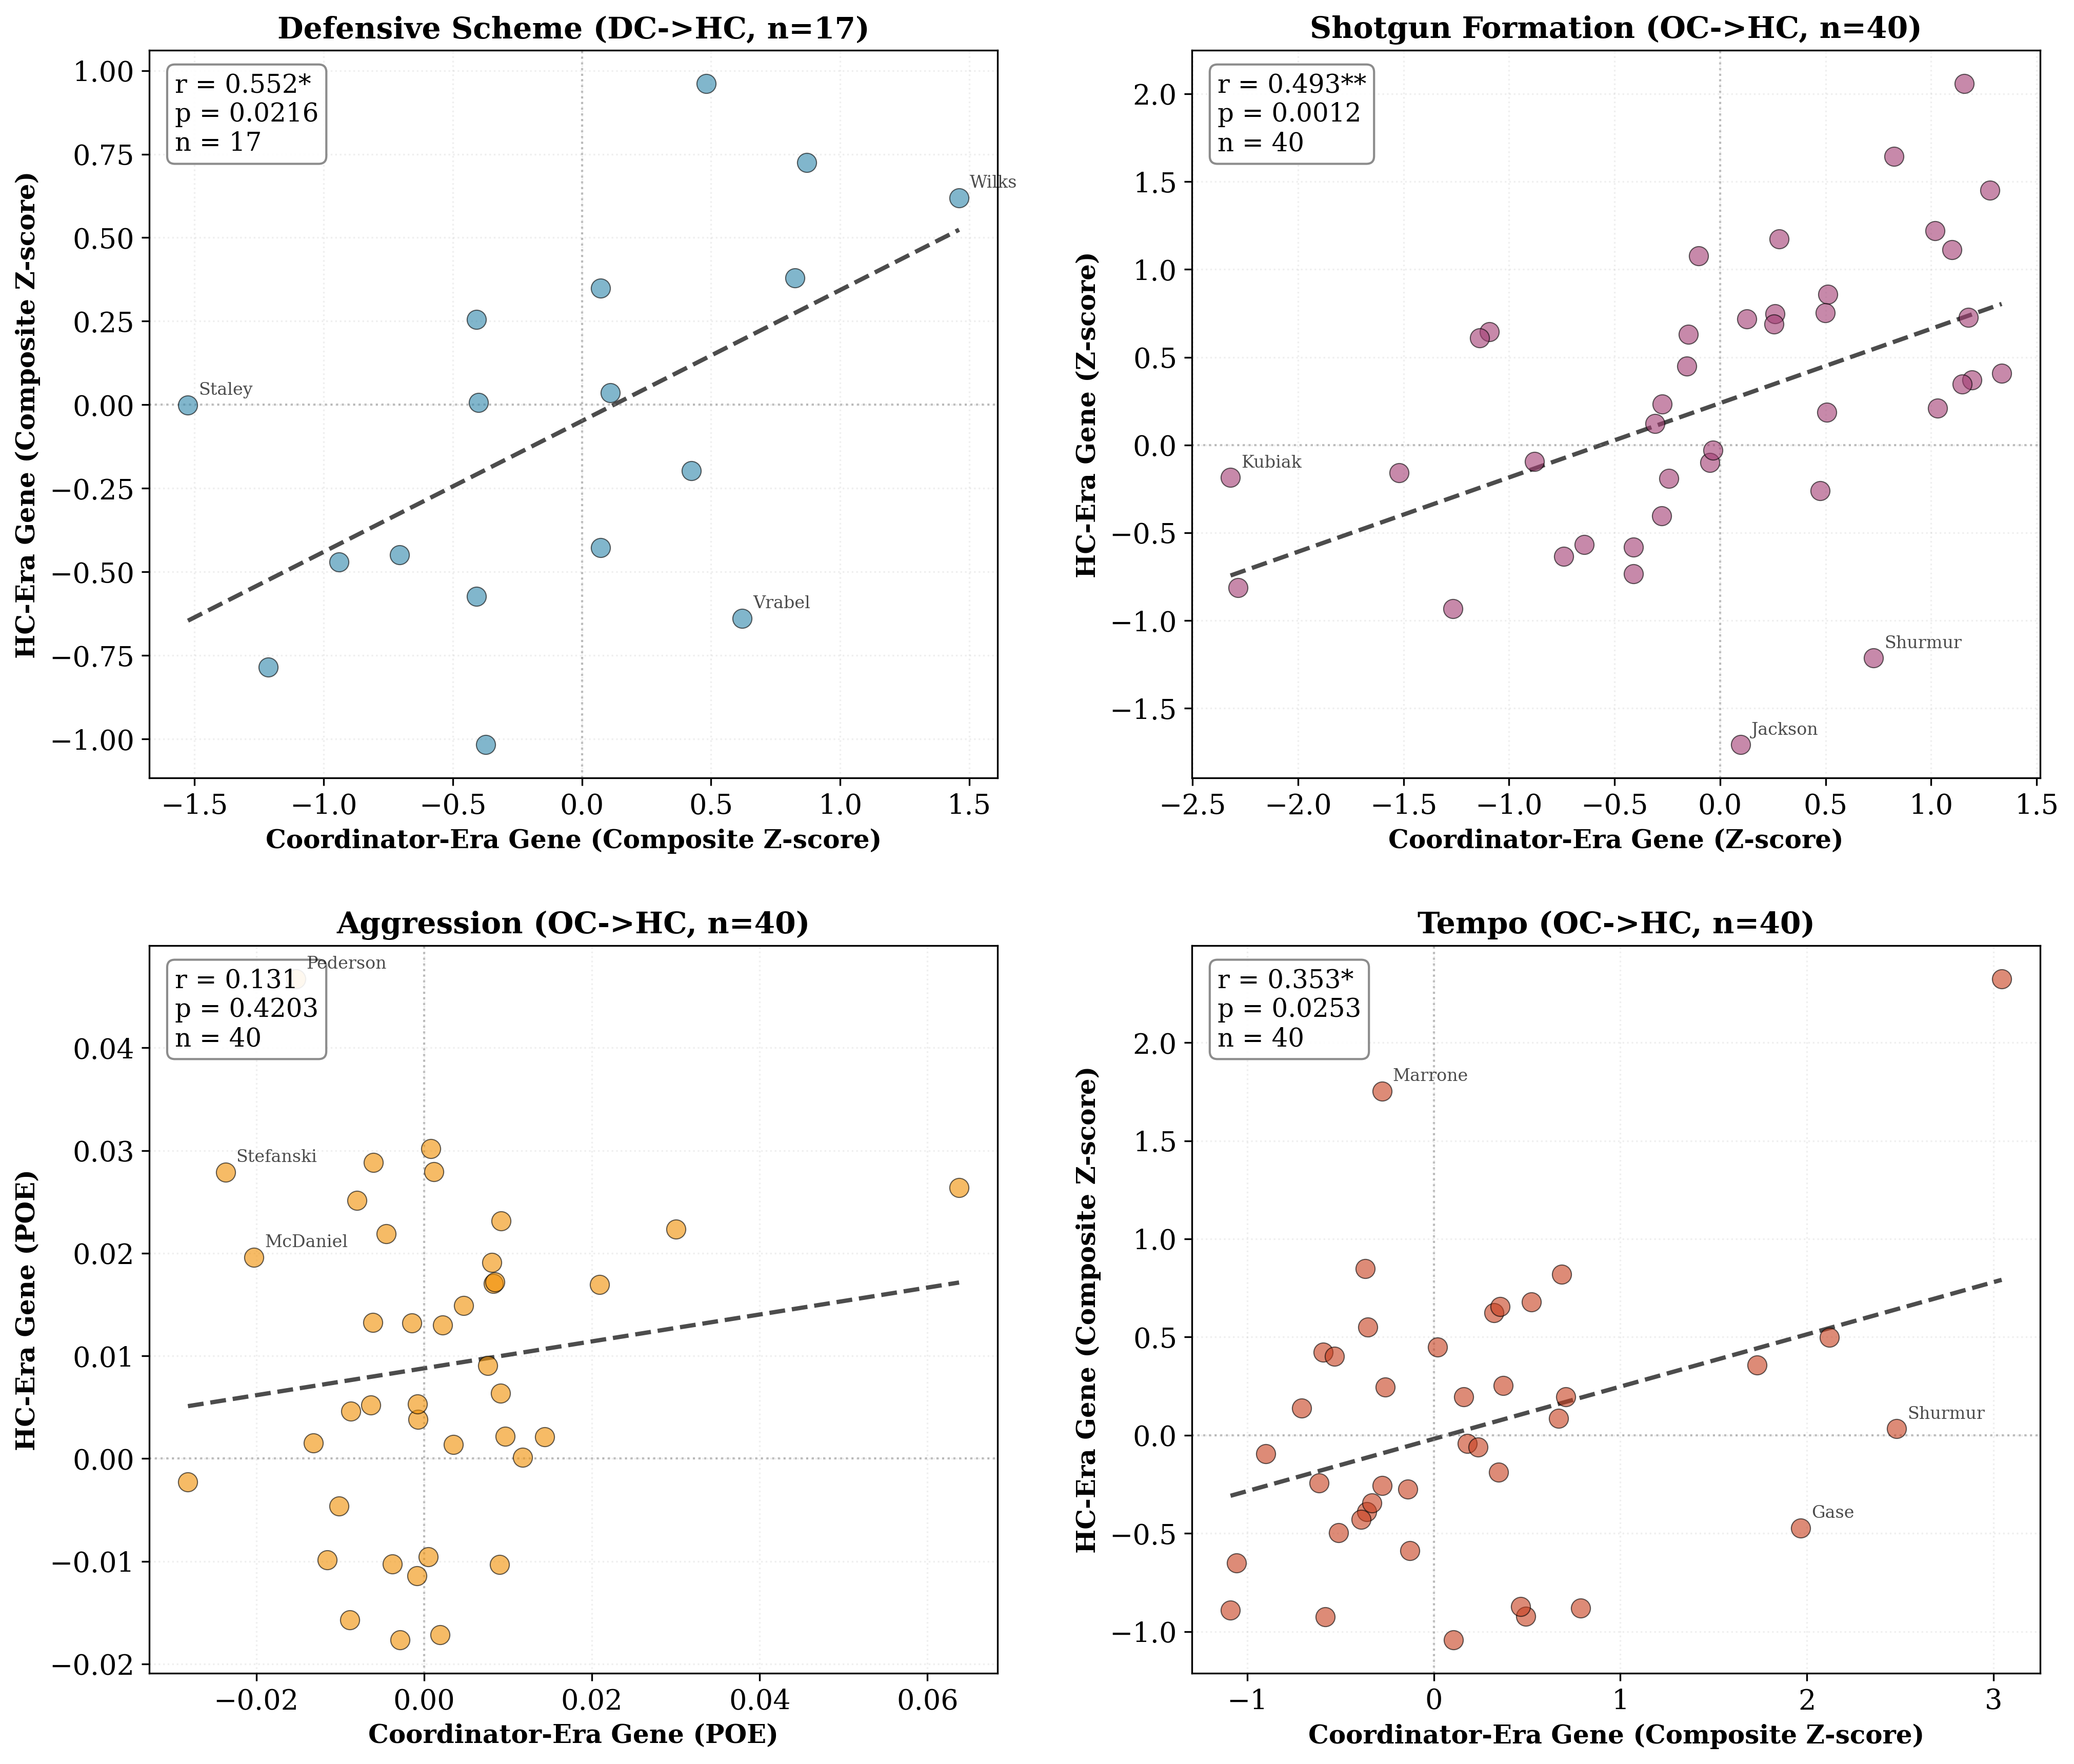
\includegraphics[width=\textwidth]{../visualizations/inheritance/gene_inheritance_scatter.png}
    \caption{Coordinator-era gene versus HC-era gene for all four dimensions. Each point represents one coordinator-to-HC transition. Shotgun formation and defensive aggression show strong positive correlations, indicating that schematic identity persists. Offensive Aggression shows no relationship and tempo only a weak, statistically unreliable one, indicating that situational decision-making and pace do not reliably transfer.}
    \label{fig:gene_scatter}
\end{figure}

Figure~\ref{fig:gene_summary} summarizes the inheritance strength and direction retention across all four genes.

\begin{figure}[H]
    \centering
    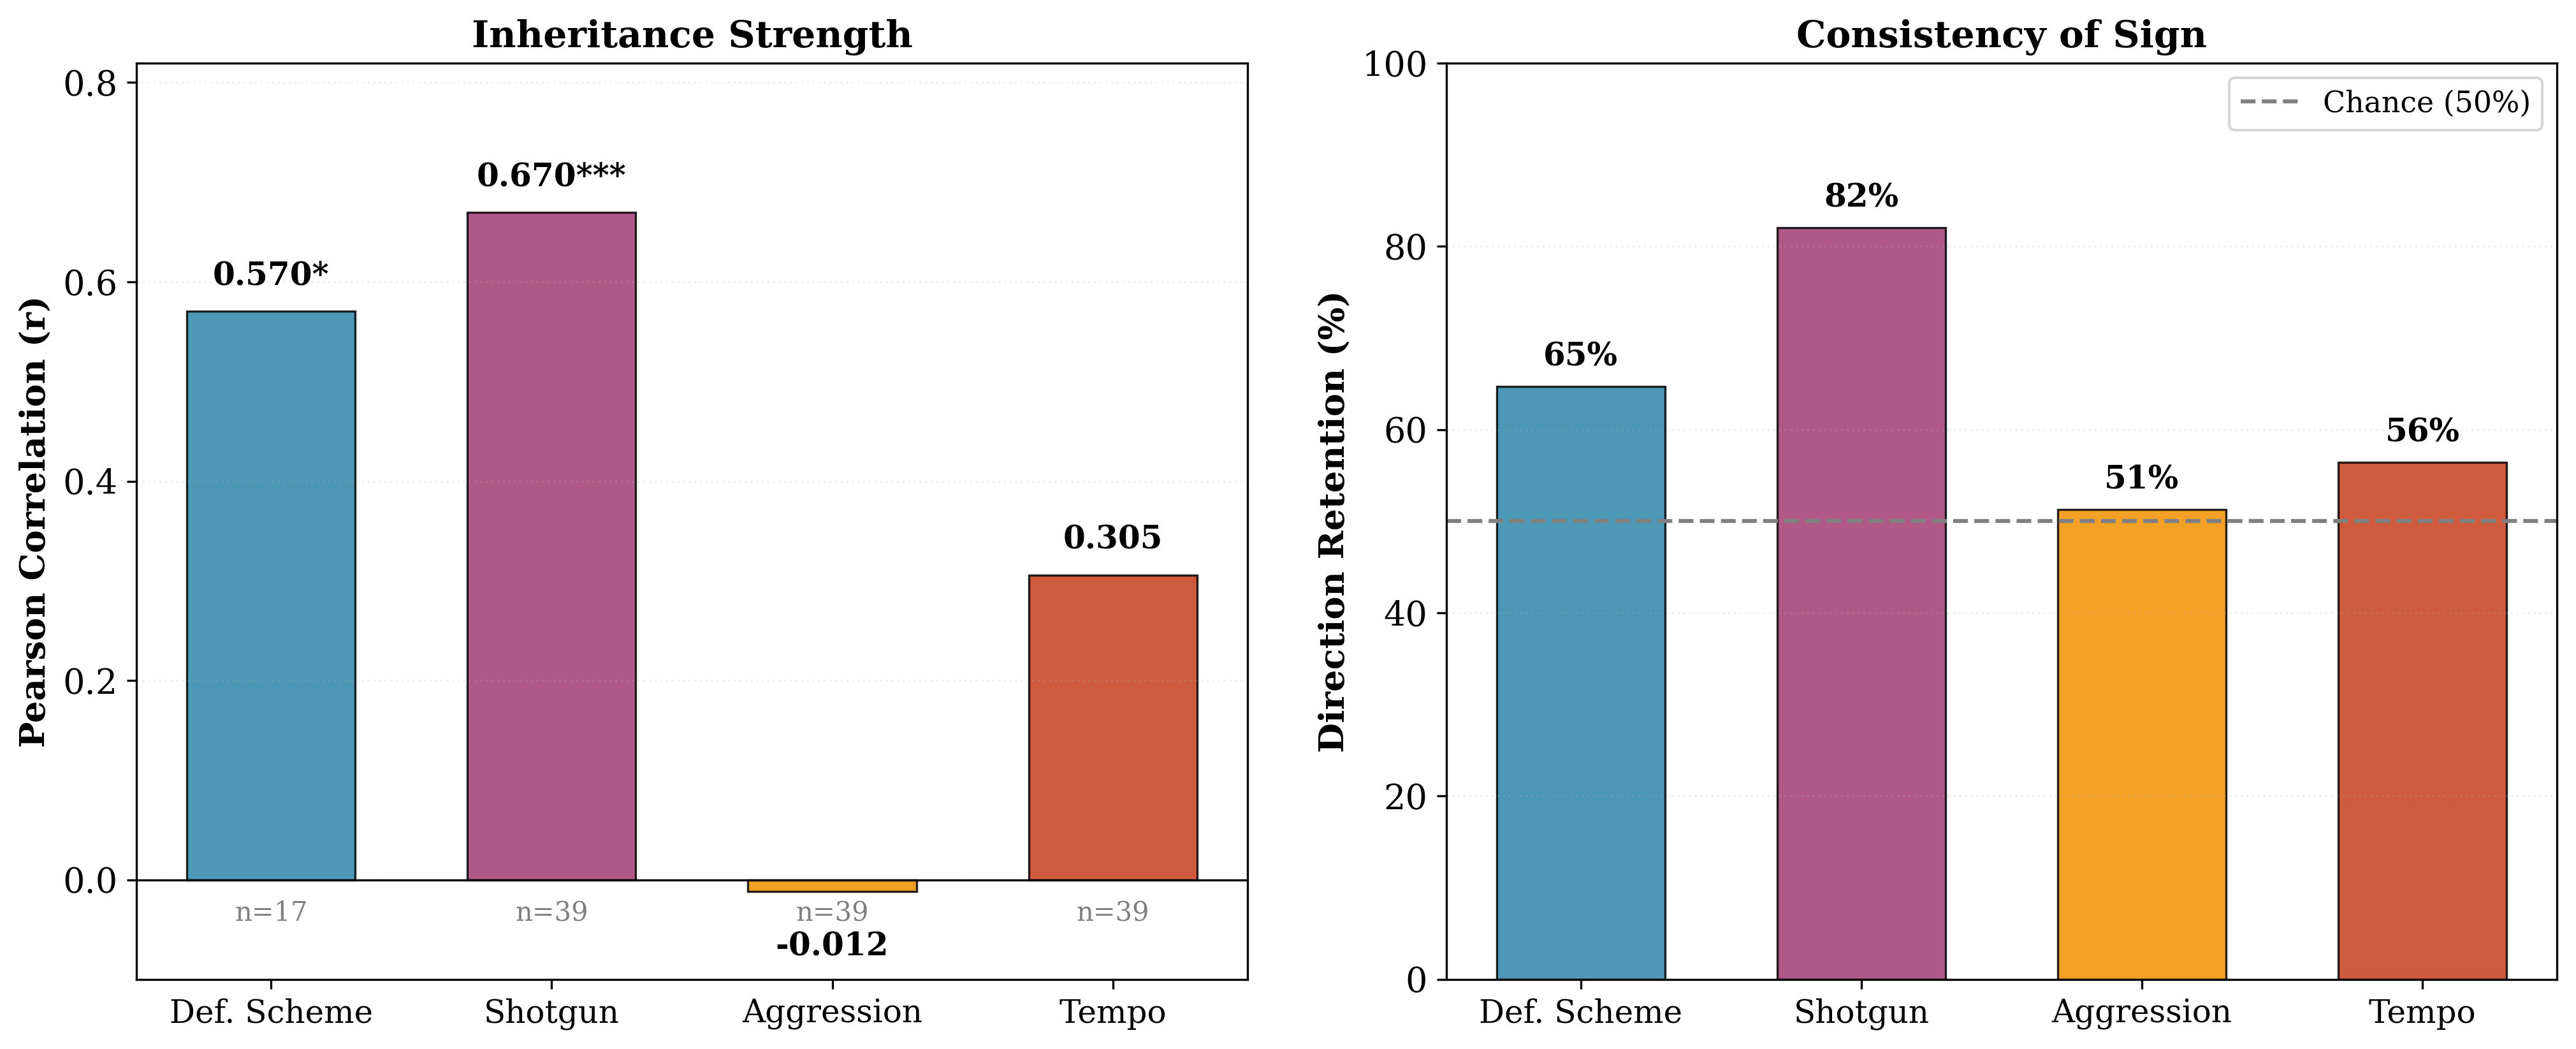
\includegraphics[width=\textwidth]{../visualizations/inheritance/gene_inheritance_summary.png}
    \caption{Left: Pearson correlation between coordinator-era and HC-era genes. Right: Percentage of coaches whose gene retains the same sign (positive/negative) across transitions. The dashed line indicates chance level (50\%). Schematic genes (defensive aggression, shotgun) show strong inheritance while situational decision-making (offensive aggression) and tempo do not.}
    \label{fig:gene_summary}
\end{figure}

\subsubsection{Synthesis: What Coaching Trees Actually Transmit}

Table~\ref{tab:tree_summary} synthesizes the coaching tree findings across all dimensions tested.

\begin{table}[H]
\caption{Summary: What Coaching Trees Transmit}
\label{tab:tree_summary}
\begin{tabular}{llccc}
\toprule
\textbf{Dimension} & \textbf{Type} & \textbf{r} & \textbf{95\% CI} & \textbf{Transmitted?} \\
\midrule
Performance (WAR), mentor $\to$ prot\'{e}g\'{e} & Outcome & 0.12 & [$-$0.01, 0.26] & No \\
Offensive Aggression (composite) & Situational & 0.02 & [$-$0.11, 0.16] & No \\
Shotgun (offensive mentor $\to$ his OC) & Schematic & 0.41 & [0.17, 0.60] & Yes \\
Shotgun (direct OC $\to$ HC) & Schematic & 0.63 & [0.48, 0.77] & Yes \\
Defensive Aggression (DC $\to$ HC) & Schematic & 0.56 & [0.19, 0.83] & Yes \\
\midrule
\multicolumn{5}{l}{\small Contemporary-group (era) adjusted, mentor- or coach-clustered. The shotgun}\\
\multicolumn{5}{l}{\small offensive-mentor-to-DC cell and the pooled correlation fall to near zero once era}\\
\multicolumn{5}{l}{\small is removed; transmission is the offensive-coordinator apprenticeship specifically.}\\
\bottomrule
\end{tabular}
\end{table}

The pattern across dimensions is consistent. Coaching trees show no transmission of performance or general risk tolerance, but offensive coaching trees \emph{do} transmit schematic identity through one specific channel: a mentor's own offensive coordinators inherit his formation tendencies (shotgun), and the same shows up in the direct coordinator-to-head-coach transitions (Table~\ref{tab:gene_inherit}). Once era is controlled, the apparent diffuse transmission turns out to have been the shared league trend, not apprenticeship. The distinction maps onto system design (transmissible, and only by those who designed it) versus situational judgment (personal). It also sets up the central asymmetry of the next section: the gene that transmits most strongly, shotgun, is \emph{not} the gene that predicts winning, offensive aggression. Coaching trees propagate systems, not the edge.

\subsection{Offensive Aggression and Performance: A Disappearing Advantage}

At the season level, where our temporal tests operate, the composite offensive aggression-WAR relationship is positive overall ($r=0.19$ raw, $0.16$ era-adjusted; Table~\ref{tab:gene_war}) but changes across the window. Table~\ref{tab:overall_war} presents the raw component relationships pooled across 2006-2024; the era split that follows is itself a within-era control.

\begin{table}[H]
\caption{Offensive Aggression vs. WAR: Overall (2006-2024)}
\label{tab:overall_war}
\begin{tabular}{lccc}
\toprule
\textbf{Measure} & \textbf{r} & \textbf{95\% CI} & \textbf{P-value} \\
\midrule
Composite & 0.189 & [0.10, 0.28] & $<$0.001 \\
\cmidrule{1-4}
Pass-Heavy & 0.183 & [0.07, 0.28] & 0.002 \\
4th Down & 0.095 & [0.01, 0.18] & 0.033 \\
Deep Pass & 0.020 & [$-$0.07, 0.11] & 0.65 \\
2-Point & 0.037 & [$-$0.06, 0.13] & 0.45 \\
\midrule
\multicolumn{4}{l}{\small N=608 coach-years; coach-clustered bootstrap p and 95\% CI}\\
\bottomrule
\end{tabular}
\end{table}

Composite offensive aggression is positively related to performance ($r=0.189$, 95\% CI $[0.10, 0.28]$, $p<0.001$), driven primarily by the pass-heavy component ($r=0.183$, $[0.07, 0.28]$, $p=0.002$); the fourth-down component is positive but weaker ($r=0.095$, $[0.01, 0.18]$, $p=0.033$), and stronger at the career level ($r=0.187$). Splitting the sample into three eras (2006-2011, $n=192$; 2012-2017, $n=192$; 2018-2024, $n=224$) reveals a decline (Table~\ref{tab:era_war}).

\begin{table}[H]
\caption{Offensive Aggression vs. WAR by Era}
\label{tab:era_war}
\small
\begin{tabular}{lccc}
\toprule
\textbf{Era} & \textbf{Composite (r [95\% CI], p)} & \textbf{Pass-Heavy (r [95\% CI], p)} & \textbf{N} \\
\midrule
2006-2011 & 0.239 [0.07, 0.38], 0.001 & 0.173 [0.00, 0.32], 0.016 & 192 \\
2012-2017 & 0.137 [$-$0.07, 0.29], 0.059 & 0.175 [0.01, 0.32], 0.015 & 192 \\
2018-2024 & 0.101 [$-$0.03, 0.25], 0.132 & 0.131 [$-$0.04, 0.31], 0.049 & 224 \\
\midrule
\multicolumn{4}{l}{\small Unclustered subgroup p; 95\% CIs are coach-clustered bootstrap}\\
\bottomrule
\end{tabular}
\end{table}

Composite offensive aggression's edge roughly halved across the window, from $r=0.239$ (95\% CI $[0.07, 0.38]$, $p=0.001$) in the early era to $r=0.137$ ($[-0.07, 0.29]$, $p=0.059$) in the middle and $r=0.101$ ($[-0.03, 0.25]$, $p=0.13$) in the modern era. The advantage diminished rather than vanished: the pass-heavy component in particular remains positive even in the modern era ($r=0.131$, $[-0.04, 0.31]$, $p=0.049$). This erosion coincides with a leaguewide shift in the tactic itself (Figure~\ref{fig:adoption}): mean composite offensive aggression climbed from below the model's season-agnostic baseline early, crossing it around 2013, to clearly above it by the modern era, and its spread across coaches widened by about a fifth, the diffusion pattern one expects as an edge becomes common knowledge.

\begin{figure}[H]
    \centering
    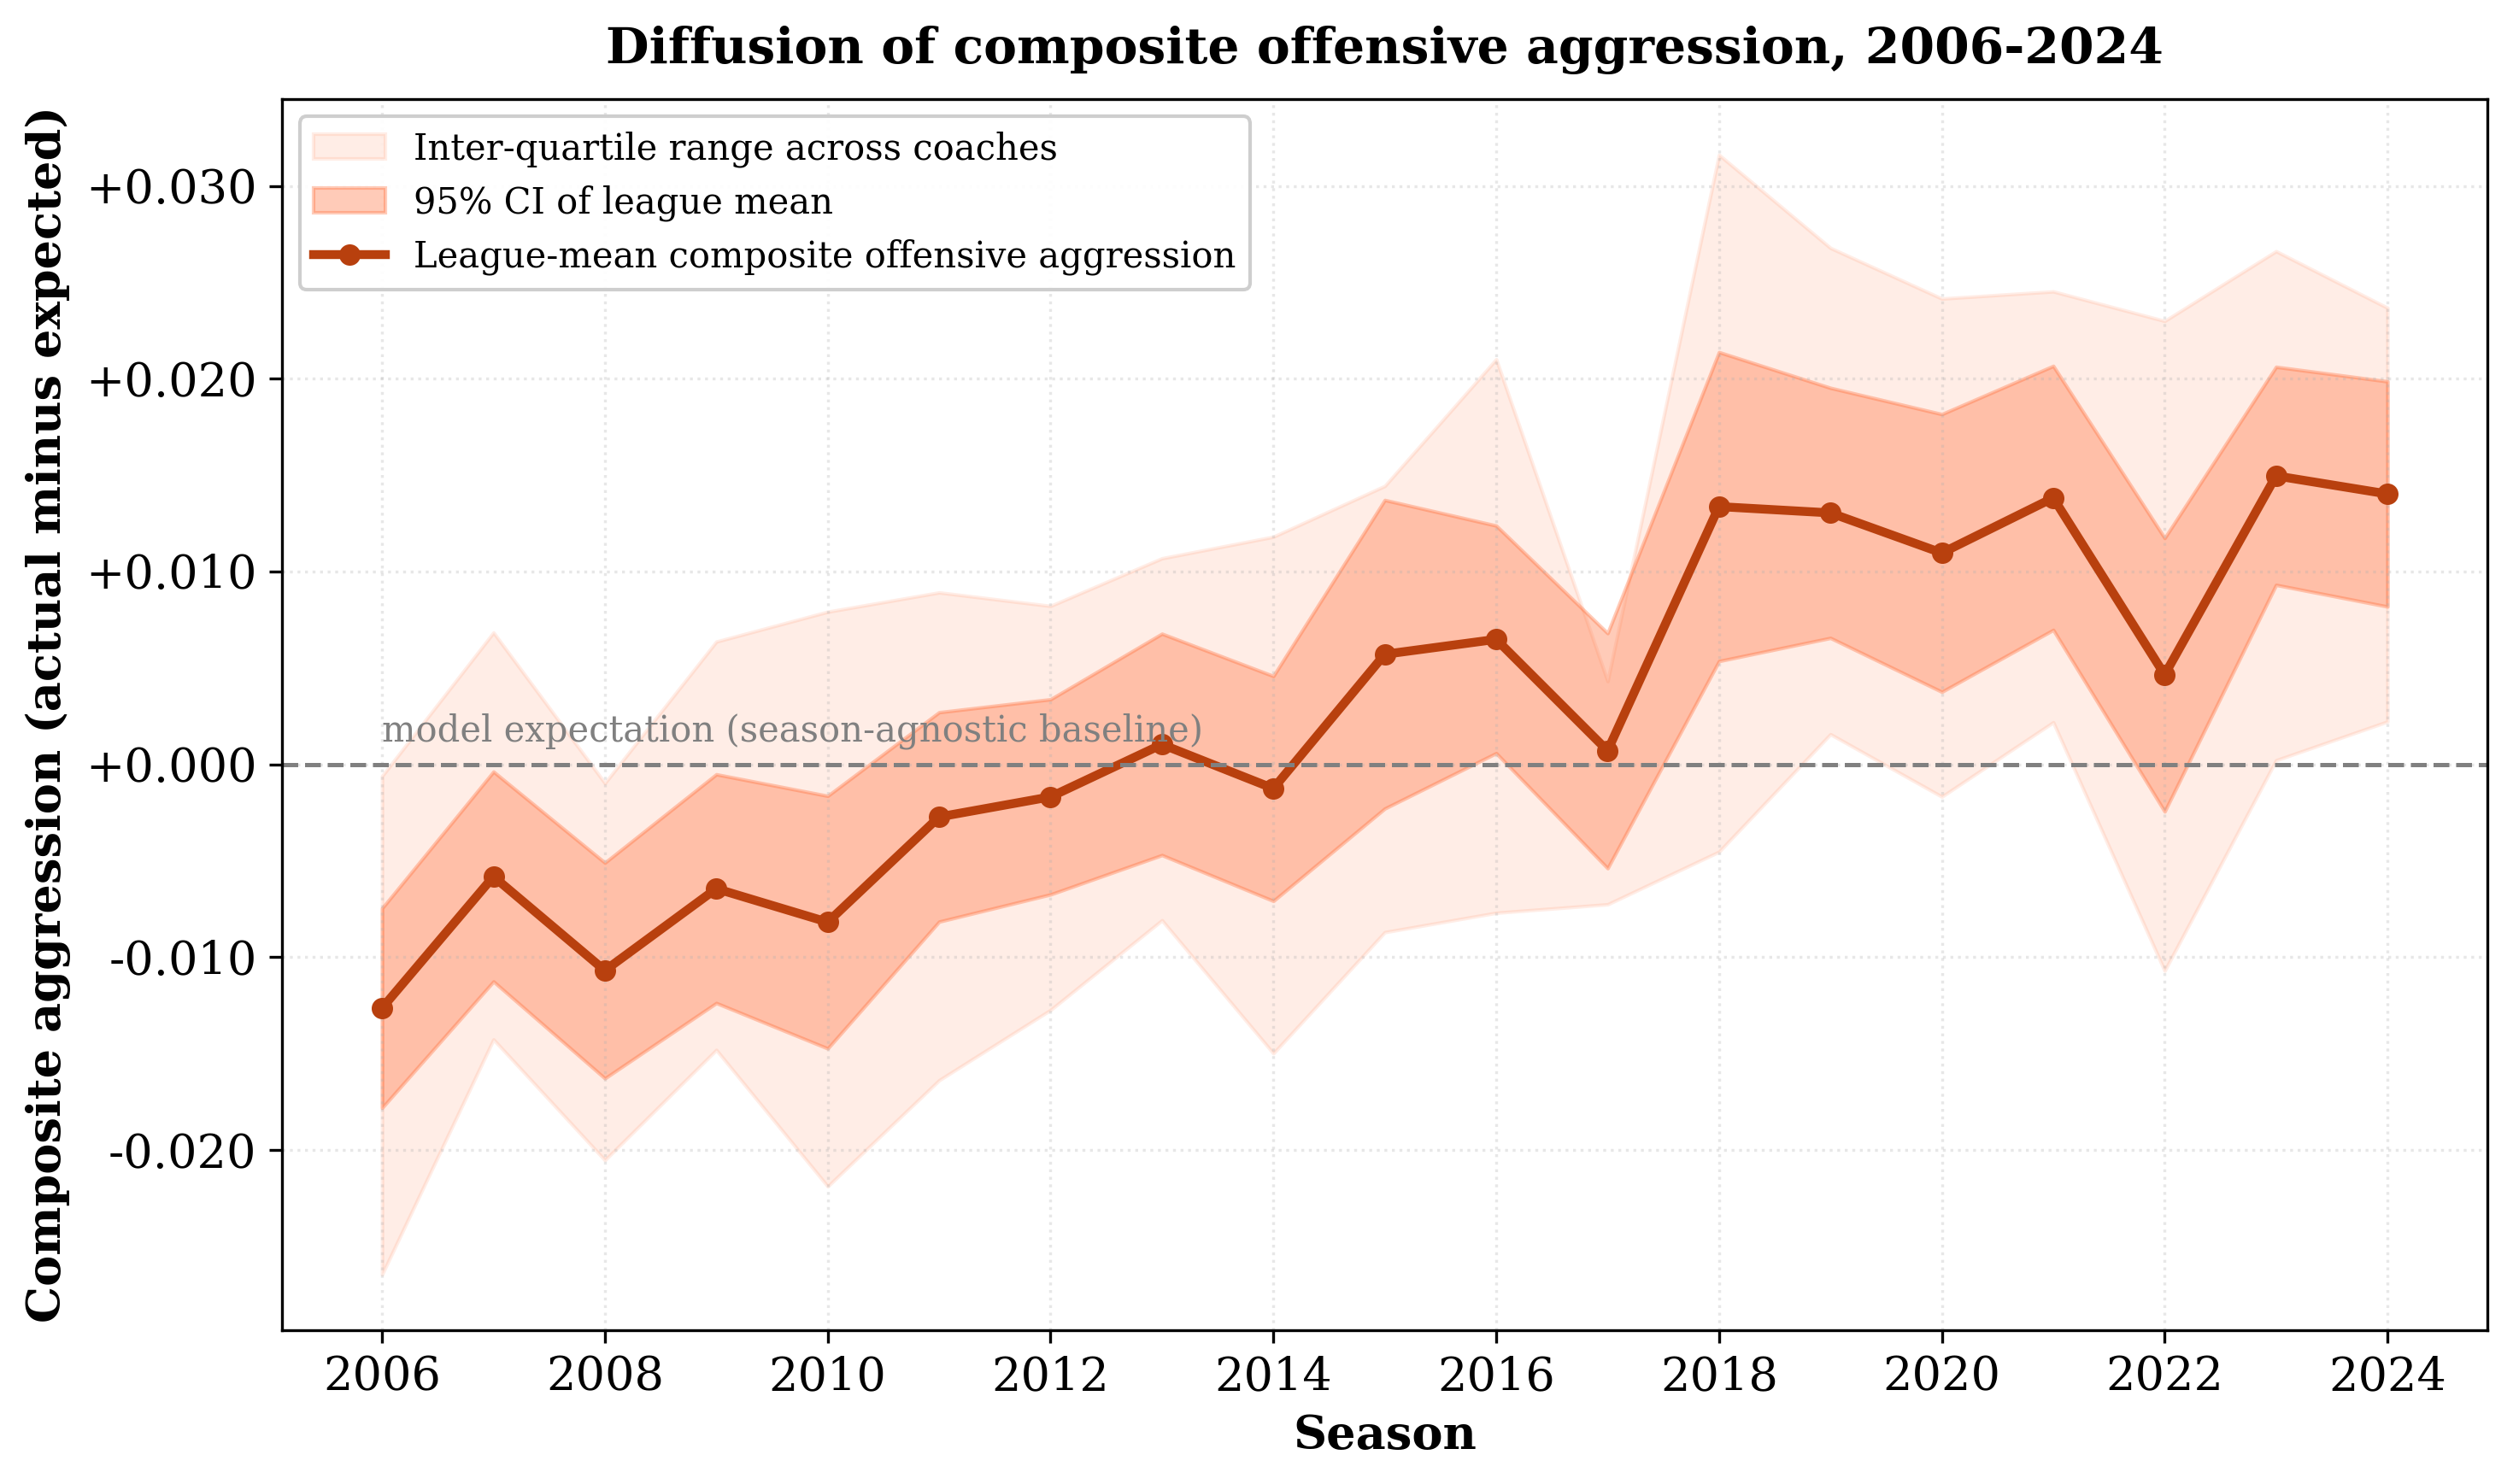
\includegraphics[width=0.85\textwidth]{../visualizations/performance/aggression_adoption_curve.png}
    \caption{Diffusion of composite offensive aggression, 2006--2024. The league-mean composite offensive aggression gene (actual minus the season-agnostic model expectation, reliability-weighted across the four sub-components; dark line, 95\% CI shaded) rises from below the time-invariant baseline in the early era, crossing it around 2013, to clearly above it by the modern era, while the inter-quartile range across coaches (light band) widens. Because the baseline model excludes season, the upward drift is the adoption signal: average aggression rose and coaches spread out in how far they pushed it.}
    \label{fig:adoption}
\end{figure}

This erosion is real but partial rather than a clean disappearance, and our robustness checks qualify it accordingly. A continuous year-by-aggression interaction is negative, consistent with decline, but its confidence interval includes zero ($\beta_3 = -0.88$, 95\% CI $[-2.36, 0.59]$), so the continuous test alone is not decisive; the implied effect fades from $\beta = 25.1$ in 2006 to $\beta = 9.2$ in 2024 rather than reversing sign. A Chow test points to a structural break around 2012, with the offensive aggression coefficient falling 61\% ($\beta = 27.2 \rightarrow 10.7$; a 2013 break is comparable), though both breaks sit just above our strict false-discovery threshold and so are suggestive. An out-of-sample check agrees: fit on 2006--2018 and applied to 2019--2024, the season-level offensive aggression-WAR relationship generalizes only weakly (test $r=0.12$), as expected when the outcome is dominated by single-season luck.

The relationship holds across coach backgrounds. Offensive aggression predicts WAR similarly for offensive-minded and defensive-minded head coaches ($r=0.21$, $[0.09, 0.33]$, and $r=0.18$, $[0.02, 0.33]$). Defensive aggression, by contrast, relates to WAR only for offensive-minded coaches ($r=0.15$, $[0.01, 0.30]$) and not defensive-minded ones ($r=0.03$, $[-0.14, 0.21]$), a counterintuitive contrast we read cautiously given the small defensive-coach sample ($n=29$ coaches).

\subsubsection{Within-Coach Fixed Effects: Causal Evidence}

Does offensive aggression cause better performance, or do better coaches simply become more aggressive? To address this, we employ two-way fixed effects regression controlling for both coach quality and temporal trends. The within-coach approach compares each coach to themselves across different years, isolating behavioral effects from selection confounds.

Table~\ref{tab:fixed_effects} presents the results. A two-way fixed-effects specification that demeans offensive aggression within both coach and year, which by construction also removes the leaguewide era trend, indicates a positive within-coach effect ($p<0.001$). Being more aggressive than one's own norm is associated with better performance, not simply a matter of better coaches happening to be more aggressive. On the same 2+season sample and WAR-games scale as the effect-size analysis, a one within-coach standard deviation increase in offensive aggression corresponds to 0.34 additional WAR games (Cohen's $d=0.21$), about 14\% of the IQR in the WAR distribution (2.52 games), with 99\% power in the pooled sample.

\begin{table}[H]
\caption{Within-Coach Fixed Effects: Offensive Aggression $\rightarrow$ WAR}
\label{tab:fixed_effects}
\begin{tabular}{lcccc}
\toprule
\textbf{Sample} & \textbf{Within-coach $\beta$} & \textbf{95\% CI} & \textbf{p} & \textbf{n} \\
\midrule
\textbf{Pooled (2006-2024)} & 22.4 & [12.1, 31.4] & $<$0.001 & 587 \\
\midrule
\multicolumn{5}{l}{\small Two-way fixed effects (offensive aggression demeaned within coach and year, the}\\
\multicolumn{5}{l}{\small latter an era control), coach-clustered SEs with a coach-block bootstrap 95\% CI;}\\
\multicolumn{5}{l}{\small 103 coaches. $\beta$ is WAR games per unit of the composite gene; equivalently}\\
\multicolumn{5}{l}{\small 0.34 games per within-coach SD (Cohen's $d=0.21$, 14\% of the 2.52-game IQR,}\\
\multicolumn{5}{l}{\small 99\% power).}\\
\bottomrule
\end{tabular}
\end{table}

We report the pooled within-coach estimate, which is the most reliable (99\% power). Era-stratified within-coach estimates are far noisier and do not follow a monotone trend, so they neither confirm nor rule out erosion of the within-coach effect.



\section{Discussion}

\subsection{The Erosion of a Competitive Advantage}

Aggressive play-calling provided a measurable edge in 2006-2011 ($r=0.239$, 95\% CI $[0.07, 0.38]$, $p=0.001$) that diminished to $r=0.101$ ($[-0.03, 0.25]$, $p=0.13$) by 2018-2024. The continuous year-by-aggression interaction is negative but imprecise ($p=0.24$), and the 2012 structural break ($p=0.03$) is modest on its own; together with the era pattern, this points to a partial erosion that we treat as suggestive rather than firmly established. As analytics-driven decision-making spread, aggressive tactics became more common: composite offensive aggression moved from below baseline on average in the early era to above baseline by the modern era, and its dispersion across coaches widened by about a fifth, suggesting experimentation as the tactic diffused. Whether the residual erosion reflects defensive adaptation (counter-strategies against predictable offensive aggression) or competitive equilibration (offensive aggression becoming table stakes) remains ambiguous.

\subsection{Causality: Evidence from Within-Coach Variation}

Our two-way fixed effects analysis provides evidence that the offensive aggression-performance relationship is at least partly causal. By comparing each coach to themselves across years, we find that a one within-coach standard deviation increase in offensive aggression corresponds to 0.34 additional WAR games (two-way fixed effects $p<0.001$, Cohen's $d=0.21$), even after removing all between-coach differences and temporal trends, the year fixed effect itself serving as an era control. The relationship is not simply that better coaches happen to be more aggressive. Within the same coach, being more aggressive predicts better performance.

However, era-stratified within-coach estimates do not follow a monotone trend, preventing us from confirming whether this within-coach effect has eroded. Three findings converge on a causal interpretation. Cross-sectional correlations are strongest when tactics were rare, the relationship erodes as tactics spread, and a within-coach effect persists after controlling for stable characteristics. For practitioners, the practical reading is that offensive aggression's edge has narrowed to at most a weak association in the modern era.

\subsection{Scheme Identity vs. Situational Decision-Making}

Our analyses reveal a clean dissociation between what coaching trees transmit and what predicts winning. \emph{Schematic identity}, the formation tendencies captured by shotgun usage, transmits through the offensive-coordinator apprenticeship (a mentor's own offensive coordinators, $r=0.41$; direct coordinator-to-head-coach, $r=0.63$) but, once the leaguewide trend is removed, does not by itself predict performance (season-level $r=0.08$, not distinguishable from zero; the career-level $0.23$ was inflated by an observation-window era artifact). \emph{Situational decision-making}, the in-game risk choices captured by offensive aggression, is the mirror image: it predicts performance (era- and noise-adjusted $r=0.18$, $p=0.003$) but does not transmit through coaching trees (near zero in every cell). The heritable offensive trait is not the adaptive one, and the adaptive one is the least heritable.

Defensive aggression is the one gene that does both, transmitting from coordinator to head coach ($r=0.56$) while also relating to WAR ($r=0.15$), though on the shorter 2016--2024 window and with the reverse-causation caveat noted below. The broader pattern echoes a familiar point from quantitative genetics: heritability and fitness are distinct properties of a trait. A tendency can pass reliably from one coaching generation to the next without being the thing that wins games, and the thing that wins games can be a personal trait that does not propagate. Transmission is also domain-specific, since only offensive coordinators, who design and install formation packages, pass on offensive scheme; the defensive-coordinator prot\'{e}g\'{e}s of the same mentors do not, and their apparent inheritance was era co-drift. This is consistent with coaching DNA propagating through expertise rather than mere exposure.

The dissociation also surfaces within offensive aggression. Fourth-down philosophy is among the most persistent components within a coach (Table~\ref{tab:persistence}), arguably its most schematic facet given that teams develop explicit decision charts, yet its cross-coach inheritance is essentially nil once era and mentor clustering are applied. Pass-heavy and two-point tendencies are more reactive to game flow.

\subsection{Challenging the Coaching Tree Narrative}

The coaching tree narrative shapes NFL hiring decisions, but our data sit uneasily with its premises. Mentor WAR shows at most a weak association with prot\'{e}g\'{e} WAR ($r=0.124$, 95\% CI $[-0.01, 0.26]$, $p=0.087$), giving little indication that working under a successful coach makes a coach successful. Composite offensive aggression shows no transmission once era is controlled ($r=0.02$, $[-0.11, 0.16]$). For success and situational decisions alike, the premises of pedigree-based hiring find little support here.

However, offensive coaching trees \emph{do} transmit schematic identity, through one specific channel. An offensive mentor's own offensive coordinators inherit his shotgun formation tendencies ($r=0.41$, $p=0.005$), and the direct coordinator-to-HC analysis indicates that formation preferences ($r=0.63$) and defensive aggression ($r=0.56$) persist through promotion, both robust to the era control, while pace does not. When Matt Nagy left Kansas City's shotgun-heavy offense to coach Chicago, he installed a nearly identical formation philosophy. When Dan Quinn left Dallas's aggressive defense to coach Washington, his defense looked similar. Teams can reliably predict the \emph{system} a coordinator will install. But that system is not itself a performance edge, since shotgun identity does not predict WAR once era is controlled, so what transmits down the tree is style, not winning.

\subsection{Limitations}

Several limitations warrant discussion beyond the causality concerns addressed earlier.

First, our play-by-play data begin in 2006, missing earlier eras. We cannot determine whether the early aggressive advantage we observe in 2006-2011 was itself a continuation of an even longer trend or represented a genuine inflection point. Historical data would reveal whether similar adoption curves occurred for previous innovations.

Second, our inheritance analyses are limited by sample size. The career-average mentor-prot\'{e}g\'{e} analysis uses 192 unique pairs for offensive aggression and 228 for shotgun, and within the $2\times2$ the key offensive-mentor-to-OC cell rests on 40--45 pairs; the direct coordinator-to-HC analysis uses 17--40 transitions. The defensive aggression analysis is particularly constrained ($n=17$) because defensive tracking data only became available in 2016. We address the small-cluster regime with wild cluster bootstrap p-values below 40 clusters. Even so, the shotgun coordinator-to-HC result ($n=40$, era-adjusted $r=0.63$, $p<0.001$) is robust, and the offensive-mentor-to-OC apprenticeship cell ($n=45$, $r=0.41$, $p=0.005$) corroborates the pattern, whereas the defensive-aggression transition ($n=17$) should be read as suggestive. The cross-team travel test, at only 32 movers, is similarly underpowered once era is removed and we lean on it lightly.

Third, the gene-WAR correlations should be interpreted with caution regarding causality. The defensive aggression-WAR correlation (era-adjusted season-level $r=0.15$, 95\% CI $[0.03, 0.27]$) may reflect reverse causation: teams with better defensive talent can afford to play man coverage and send extra rushers, whereas the gene framework attributes this to coaching philosophy. Our residual approach controls for game situation but cannot fully separate this preference from roster-enabled opportunity.

Fourth, we cannot observe coaching constraints. Some coaches may want to be aggressive but face organizational pressure to be conservative. Others may have coordinator partnerships that override their personal preferences. Our measures capture observed behavior rather than underlying intentions, which may differ due to unmeasured constraints.

Fifth, the season-level gene-WAR estimates require two adjustments, which we treat as a single design rather than as separate caveats. Single-season WAR is noisy (year-over-year reliability about one-quarter), so we inverse-variance weight by games-based precision rather than collapsing to careers; and because a leaguewide baseline drifts over our window, we remove each season's mean before correlating, the standard contemporary-group adjustment of quantitative genetics. The career-average correlation is reported only as a secondary anchor, since within a fixed observation window it acquires a selection-driven era component (career-mean WAR versus era $r\approx0.30$) that inflates it. This control changes one earlier conclusion: shotgun formation preference, which appeared to predict WAR at the career level, does not once era is removed, so we reclassify it as a transmissible but not directly performance-relevant trait. A reader who regarded the leaguewide drift as part of a gene's value would weight the raw estimates more heavily; we report both throughout.

Sixth, we attribute each gene to the head coach as the accountable decision-maker, yet play-calling responsibility varies: some head coaches call their own offensive or defensive plays while most delegate to a coordinator. This introduces idiosyncratic noise into the attribution rather than systematic bias, and the strong face validity and cross-team portability of the genes indicate that head-coach attribution nonetheless captures genuine coach-specific signal. Relatedly, the defensive-aggression gene is measured at the team level and so blends head coach, coordinator, and personnel.

Finally, ``offensive aggression'' is best understood as a formative index of four weakly-correlated facets (fourth-down, pass-run balance, deep passing, two-point) rather than a single latent trait; we therefore report the components alongside the composite, and note that the composite-WAR relationship is carried mainly by the pass-heavy and fourth-down facets.

\section{Conclusion}

Through analysis of more than 600,000 plays and 608 coach-years (2006--2024), we develop a machine learning framework for measuring coaching ``DNA'' across four strategic dimensions and test what this DNA is, what it predicts, and how it transmits.

First, coaching genes are genuine, stable traits of the coach rather than artifacts of the team. Coach identity explains several times as much of each gene's variance as team identity, even net of a permutation null, and when coaches change teams their strategic tendencies travel with them (composite offensive aggression $r=0.57$, 95\% CI $[0.33, 0.74]$, across team changes), with rankings that match public reputation. This grounds the rest of the analysis: the genes measure the coach.

Second, the genes that predict performance are the aggression measures. Once both WAR noise and the leaguewide era trend are controlled at the season level, composite offensive aggression ($r=0.18$, $p=0.003$) and defensive aggression ($r=0.15$, $p=0.014$) predict WAR, while shotgun and tempo do not; shotgun's apparent career-level edge ($r=0.23$) was an observation-window era artifact. The offensive aggression edge has also diminished over time, from $r=0.24$ (2006--2011) to $r=0.10$ (2018--2024), with a modest 2012 structural break ($p=0.03$), as analytics-driven tactics spread.

Third, coaching trees transmit systems, not success or risk tolerance. Mentor WAR shows at most a weak association with prot\'{e}g\'{e} WAR ($r=0.124$, $p=0.087$), and composite offensive aggression shows no inheritance once era is controlled ($r=0.02$). But schematic identity transmits through the offensive-coordinator apprenticeship specifically: a mentor's own offensive coordinators inherit his shotgun tendencies ($r=0.41$) and the direct coordinator-to-HC transition is stronger still ($r=0.63$), as is defensive aggression ($r=0.56$), all robust to era control, while the diffuse impression of inheritance was the shared league trend. Strikingly, the trait that transmits most strongly is not the one that predicts winning: organizations can far more readily predict the system a coordinator will install than whether they will win, and the system itself is not the edge.

Within-coach fixed-effects analysis adds causal support for the performance result (0.34 WAR games per within-coach standard deviation of offensive aggression; two-way fixed effects $p<0.001$), even as the cross-sectional edge has narrowed in the modern era. The frontier appears to have moved beyond offensive aggression frequency, perhaps to scheme innovation, within-game adaptation speed, or player development, dimensions we are only beginning to measure.

\begin{acknowledgement}
  This analysis builds on play-by-play data from \texttt{nfl\_data\_py} and coaching history data scraped from Pro Football Reference. Performance metrics (WAR) were calculated separately. All code and detailed methodology are available in the project repository.
\end{acknowledgement}

\begin{thebibliography}{9}

\bibitem[Benjamini and Hochberg(1995)]{benjamini1995}
Benjamini, Y. and Hochberg, Y. (1995). Controlling the false discovery rate: A practical and powerful approach to multiple testing. \emph{Journal of the Royal Statistical Society: Series B (Methodological)}, 57(1), 289--300.

\bibitem[Burke(2009)]{burke2009}
Burke, B. (2009). Fourth down study. \emph{Advanced NFL Stats} (later renamed \emph{Advanced Football Analytics}).

\bibitem[Cameron et al.(2008)]{cameron2008}
Cameron, A. C., Gelbach, J. B., and Miller, D. L. (2008). Bootstrap-based improvements for inference with clustered errors. \emph{The Review of Economics and Statistics}, 90(3), 414--427.

\bibitem[Chen and Guestrin(2016)]{chen2016}
Chen, T. and Guestrin, C. (2016). XGBoost: A scalable tree boosting system. In \emph{Proceedings of the 22nd ACM SIGKDD International Conference on Knowledge Discovery and Data Mining}, 785--794.

\bibitem[DerSimonian and Laird(1986)]{dersimonian1986}
DerSimonian, R. and Laird, N. (1986). Meta-analysis in clinical trials. \emph{Controlled Clinical Trials}, 7(3), 177--188.

\bibitem[Goff and Wisley(2006)]{goff2006}
Goff, B. L. and Wisley, T. L. (2006). Is there a managerial life cycle? Evidence from the NFL. \emph{Managerial and Decision Economics}, 27(6), 563--572.

\bibitem[Grinsztajn et al.(2022)]{grinsztajn2022}
Grinsztajn, L., Oyallon, E., and Varoquaux, G. (2022). Why do tree-based models still outperform deep learning on typical tabular data? \emph{Advances in Neural Information Processing Systems}, 35, 507--520.

\bibitem[Horowitz and Shim(2014)]{horowitz2014}
Horowitz, I. and Shim, R. (2014). The fourth down puzzle in the National Football League. \emph{Journal of the Royal Statistical Society: Series A}, 177(3), 717--733.

\bibitem[Meinshausen and B\"uhlmann(2010)]{meinshausen2010}
Meinshausen, N. and B\"uhlmann, P. (2010). Stability selection. \emph{Journal of the Royal Statistical Society: Series B (Statistical Methodology)}, 72(4), 417--473.

\bibitem[Nadeau and Bengio(2003)]{nadeau2003}
Nadeau, C. and Bengio, Y. (2003). Inference for the generalization error. \emph{Machine Learning}, 52(3), 239--281.

\bibitem[Rogers(2007)]{rogers2007}
Rogers, E. M. (2007). \emph{Diffusion of Innovations} (5th ed.). Free Press, New York.

\bibitem[Romer(2006)]{romer2006}
Romer, D. (2006). Do firms maximize? Evidence from professional football. \emph{Journal of Political Economy}, 114(2), 340–365.

\bibitem[Schatz(2003)]{schatz2003}
Schatz, A. (2003). DVOA (Defense-adjusted Value Over Average) metrics. \emph{Football Outsiders}.

\bibitem[Sportico(2024)]{sportico2024}
Sportico (2024). Highest-paid coaches 2024: Reid, Payton, Kerr on top. \emph{Sportico}. Retrieved from https://www.sportico.com/

% Self-citation anonymized for blind peer review; restore author for camera-ready
%\bibitem[Williamson(2026)]{williamson2026war}
%Williamson, J. (2026). Coach WAR: A counterfactual approach to evaluating NFL head coach impact in the modern era. \emph{[Journal TBD]}.
\bibitem[Author(2026)]{williamson2026war}
Author (2026). Coach WAR: A counterfactual approach to evaluating NFL head coach impact in the modern era. Venue omitted for blind review.

\bibitem[Yam and Lopez(2019)]{yam2019}
Yam, D. and Lopez, M. J. (2019). What was lost? A causal estimate of fourth down behavior in the National Football League. \emph{Journal of Sports Economics}, 20(4), 479–501.

\bibitem[Yurko et al.(2019)]{yurko2019}
Yurko, R., Ventura, S., and Horowitz, M. (2019). nflWAR: A reproducible method for offensive player evaluation in football. \emph{Journal of Quantitative Analysis in Sports}, 15(3), 163--183.

\end{thebibliography}
\end{document}
